
\documentclass[11pt,a4paper]{article}
\usepackage[a4paper,top=2.6cm,bottom=2.6cm,left=2.5cm,right=2.5cm]{geometry}
\usepackage[T1]{fontenc}
\usepackage[utf8]{inputenc}
\usepackage{newtxtext}
\usepackage{amsmath}
\usepackage{newtxmath}
\usepackage{microtype}
\usepackage{xcolor}
\usepackage{graphicx}
\usepackage{booktabs,array,tabularx,longtable,xltabular}
\usepackage{enumitem}
\usepackage[font=small,labelfont={sf,bf},labelsep=period,justification=justified,singlelinecheck=false,skip=6pt]{caption}
\usepackage[nobottomtitles*]{titlesec}
\usepackage{fancyhdr}
\usepackage{lastpage}
\usepackage{pdflscape}
\usepackage[section]{placeins}
\usepackage{tikz}
\usetikzlibrary{arrows.meta,positioning,calc}
\usepackage[most]{tcolorbox}
\usepackage[colorlinks=true,linkcolor=Accent,citecolor=Accent,urlcolor=Accent]{hyperref}


%% ── One accent colour; no colour-coded content categories ────────────────────
\definecolor{Accent}{HTML}{1F3A5F}
\definecolor{Rule}{HTML}{8A94A0}
\definecolor{DRed}{HTML}{B71C1C}   % smoke-test banner only
%% Colour names used by diagram and table code carried over from the previous
%% layout all collapse to the accent or to white, so nothing is colour-coded.
\colorlet{Navy}{Accent}\colorlet{Sky}{Accent}\colorlet{Teal}{Accent}
\colorlet{FGreen}{Accent}\colorlet{Amber}{Accent}\colorlet{Purple}{Accent}
\colorlet{Indigo}{Accent}\colorlet{TGcol}{Accent}\colorlet{QGcol}{Accent}
\colorlet{FGcol}{Accent}
\colorlet{LBg}{white}\colorlet{BBg}{white}\colorlet{GBg}{white}\colorlet{ABg}{white}
\colorlet{IBg}{white}\colorlet{RBg}{white}\colorlet{TealBg}{white}
\colorlet{NavyBg}{white}\colorlet{TabOdd}{white}

%% ── Typography: serif body, sans headings, generous leading ─────────────────
\linespread{1.12}
\setlength{\emergencystretch}{2.5em}
\setlength{\parindent}{1.2em}
\setlength{\parskip}{0.2\baselineskip}
\titleformat{\section}{\sffamily\Large\bfseries\color{Accent}}{\thesection}{0.7em}{}
\titleformat{\subsection}{\sffamily\large\bfseries\color{Accent}}{\thesubsection}{0.7em}{}
\titleformat{\subsubsection}{\sffamily\normalsize\bfseries}{\thesubsubsection}{0.6em}{}
\titleformat{\paragraph}[runin]{\sffamily\normalsize\bfseries}{}{}{}[.]
\titlespacing*{\section}{0pt}{3.4ex plus 1ex minus .2ex}{1.6ex}
\titlespacing*{\subsection}{0pt}{2.8ex plus 1ex minus .2ex}{1.2ex}
\titlespacing*{\subsubsection}{0pt}{2.2ex plus .8ex minus .2ex}{0.8ex}
\titlespacing*{\paragraph}{0pt}{1.1ex plus .5ex}{0.6em}
\setcounter{secnumdepth}{3}
\setcounter{tocdepth}{2}
\setlist{itemsep=3pt,topsep=4pt,leftmargin=1.4em}
\renewcommand{\arraystretch}{1.15}
\setlength{\textfloatsep}{14pt plus 3pt minus 3pt}
\setlength{\floatsep}{12pt plus 3pt minus 3pt}
\renewcommand{\topfraction}{0.9}\renewcommand{\textfraction}{0.08}
\renewcommand{\floatpagefraction}{0.75}

\pagestyle{fancy}
\fancyhf{}
\renewcommand{\headrulewidth}{0pt}
\fancyfoot[L]{\sffamily\footnotesize\color{Rule}Synthetic financial time series --- progress report}
\fancyfoot[R]{\sffamily\footnotesize\color{Rule}\thepage\ / \pageref{LastPage}}
\fancypagestyle{plain}{\fancyhf{}\renewcommand{\headrulewidth}{0pt}%
  \fancyfoot[R]{\sffamily\footnotesize\color{Rule}\thepage\ / \pageref{LastPage}}}

%% ── Macros ──────────────────────────────────────────────────────────────────
\newcommand{\tcite}[1]{\textsuperscript{[\hyperlink{R:#1}{#1}]}}
%% Identifiers such as \texttt{acf\_squared\_mae} may break after an underscore.
\makeatletter
\DeclareRobustCommand{\_}{\ifmmode\nfss@text{\textunderscore}\else\textunderscore\allowbreak\fi}
\makeatother
\newcommand{\E}{\mathbb{E}}
\newcommand{\norm}[1]{\left\|#1\right\|}
%% Audit rows are emitted by report_data.py; set as plain paragraphs, no box.
\newcommand{\auditrow}[5]{\par\medskip\noindent\textbf{#4}\hfill{\sffamily\footnotesize\textsc{#1}}\par\nopagebreak\noindent #5\par}

\begin{document}
%% ─── Title page ──────────────────────────────────────────────────────────────
\begin{titlepage}
\thispagestyle{empty}
\setlength{\parindent}{0pt}

\vspace*{3.2cm}
{\sffamily\color{Accent}\rule{\linewidth}{0.8pt}\par\vspace{0.9cm}
{\fontsize{30}{36}\selectfont\bfseries Synthetic Financial Time Series\par}
\vspace{0.5cm}
{\LARGE Benchmarking generative and econometric models\\[2pt] on BRICS equity indices\par}
\vspace{0.9cm}\rule{\linewidth}{0.8pt}\par}
\vspace{0.9cm}
{\sffamily\Large Progress report\par}
\vspace{2.6cm}
{\large Victor Sobottka\par}
\vspace{0.3cm}
{\normalsize Barcelona School of Economics (BSE)\\ in collaboration with Universitat Polit\`ecnica de Catalunya (UPC)\par}
\vfill
{\sffamily\small\textbf{Scope.} Five generators of daily equity returns --- three generative adversarial networks and two GARCH baselines --- trained per market on five BRICS indices, 2006--2026, and ranked with a metric suite audited against a shuffled copy of the real data.\par}
\vspace{0.7cm}
{\sffamily\small 2026-09-14\par}
\end{titlepage}
\setcounter{page}{2}

\tableofcontents
\clearpage

%% ─── Provenance ──────────────────────────────────────────────────────────────
\section*{Provenance}
\addcontentsline{toc}{section}{Provenance}
\label{sec:provenance}
Every number in this report is read from the pipeline run recorded below by \texttt{report\_data.py}; none is typed by hand. Where a statement rests on an earlier measurement that this run's artifacts do not contain, the text says so at the point it is made.

\medskip
\begin{tcolorbox}[sharp corners,boxrule=0.5pt,colframe=Rule,colback=white,
  left=8pt,right=8pt,top=6pt,bottom=6pt]
\small
\begin{tabularx}{\linewidth}{@{}>{\sffamily\bfseries}l>{\raggedright\arraybackslash}X@{}}
Generated & 2026-09-12T13:18:16 (git \texttt{a53060cc5c}) \\
Seeds & 42, 43, 44 \\
Markets & BOVESPA, FTSE, MOEX, NIFTY50, SHANGHAI \\
Walk-forward folds & 5 \\
Generator updates & 9,000 \\
Software & Python 3.12.3 $\cdot$ PyTorch 2.13.0+cu130 \\
Libraries & arch 8.0.0 $\cdot$ statsmodels 0.15.0 $\cdot$ scipy 1.18.1 $\cdot$ numpy 2.5.3 $\cdot$ pandas 2.3.3 \\
CUDA & yes (NVIDIA GeForce RTX 4090) \\
Platform & Linux-6.8.0-106-generic-x86\_64-with-glibc2.39\\
\end{tabularx}
\end{tcolorbox}

\medskip
The numerical library versions are recorded because they are load-bearing, not as bookkeeping. Whether a GARCH fit that reaches the integrated boundary generates an explosive path flipped between the production environment of an earlier run and a local refit of the same data window (Section~\ref{sec:boundary}); a difference in the \texttt{arch} version is the likeliest explanation, and that earlier run did not record it.

%% ─── Highlights ──────────────────────────────────────────────────────────────
\section{Highlights}
\label{sec:highlights}
\begin{itemize}[leftmargin=1.3em,itemsep=6pt]
\item \textbf{A 6-parameter model ranks first.} GJR-GARCH, fitted in 0.018\,s, has the best mean composite rank (2.524). The largest generator, QuantGAN, has 276,481 parameters and trains for 481\,s per market--seed, and ranks below it on composite, on fidelity and on temporal.
\item \textbf{The margin is thin, and the two families win different things.} CNN-WGAN-GP trails by 0.081 on composite. The gradient-trained family takes 10 of 15 per-evaluation composite wins and 9 of 15 fidelity wins; the econometric family takes 9 of 15 temporal wins.
\item \textbf{A shuffled copy of the real data beats most generators on volatility clustering.} 9 of 19 computed metrics cannot tell a shuffled deck from the real series at all. On the autocorrelation of squared returns the shuffled control beats all 3 GANs, and only GJR-GARCH clears it.
\item \textbf{GARCH fits reach the integrated boundary as a property of the data.} 12 of 180 econometric fits converge to persistence~1, in 4 market--window--model combinations and identically in every seed. A refit under a stationarity bound costs 0.000581 to 0.019743 in log-likelihood.
\item \textbf{Most generators remain distinguishable from real data.} In walk-forward evaluation 3 of 5 models sit more than 1.96 null standard deviations from chance on discriminative AUC. AUC falls from 0.811 to 0.664 as the training window grows, and the decline is not monotonic.
\item \textbf{Downstream, the pooled risk backtest favours CNN-WGAN-GP.} Across 3 backtests over $n$ = 2,479 pooled observations it has the lowest median QLIKE ($-$8.134).
\item \textbf{Mode collapse is caught by instrumentation, not by eye.} The post-generation guard fired 18 times across 2 models (TimeGAN (16), QuantGAN (2)); TimeGAN is the worst of the five on all 7 temporal metrics.
\end{itemize}

%% ─── Why this work matters ───────────────────────────────────────────────────
\section{Why this work matters}
\label{sec:why}
Synthetic market data is wanted where real data cannot serve: crisis episodes are too rare to train or stress-test risk models on, proprietary positions cannot be shared, and scenario analysis needs many plausible histories rather than the single one that happened. Generative adversarial networks have been proposed for this, and the reference studies --- TimeGAN\tcite{4} and QuantGAN\tcite{5} --- report that they reproduce the statistical regularities of returns, the \emph{stylised facts}\tcite{7}, better than parametric baselines.

Evaluation is the hard part. A generator can reproduce the distribution of daily returns exactly and still be useless for risk work if it scatters large moves at random, because what a risk model needs is the way turbulence clusters in time. Many of the metrics used to judge synthetic series look only at the distribution. This study measures that directly: scored by the same code as the generators, a random permutation of the real series --- identical values, no dynamics --- is indistinguishable from the real data on 9 of the 19 metrics computed here. A benchmark that does not audit its metrics against such a control cannot tell a working generator from a shuffled deck.

Emerging markets make the test harder in the ways that matter. The reference GAN studies evaluate on developed-market data, for example the S\&P~500 in Wiese et al.\tcite{5}. The five BRICS indices used here span the 2008 crisis, the 2015 Chinese market crash, the COVID shock and the suspension of the Moscow exchange in 2022, and they carry heavy tails and strong volatility clustering: across 24,758 market-days, 76 daily moves exceed five standard deviations, where a Gaussian model predicts fewer than one (Table~\ref{tab:data}). A generator that works on these series is doing something a developed-market benchmark would not reveal.

The study adds a second test that most benchmarks omit: two econometric models, GARCH(1,1)\tcite{39} and GJR-GARCH(1,1)\tcite{40}, fitted on the same data and scored by the same pipeline. A benchmark of generators against each other always produces a winner. Including the parametric baseline as a genuine competitor is what shows whether the winner is useful.
%% ─── Setting and design ──────────────────────────────────────────────────────
\section{Setting and design}
\label{sec:design}

\subsection{Data}
\label{sec:data}
The data are daily closing prices of five BRICS equity indices --- BOVESPA (Brazil), FTSE/JSE All Share (South Africa), MOEX (Russia), NIFTY~50 (India) and the Shanghai Composite (China) --- from 2006-08-30 to 2026-08-28, twenty years and 24,758 market-days of log returns in total. Each market is split in time into 80\% training, 10\% validation and 10\% test, never shuffled. Table~\ref{tab:data} summarises the returns.

\begin{table}[htbp]
\centering
\caption{The five return series, computed from the processed daily log returns. $\sigma$: daily standard deviation. Excess kurtosis is zero for a Gaussian. Residual kurtosis enters the pipeline only as a real-versus-synthetic difference, so it has no standalone value per market.}
\label{tab:data}
\begin{tabular}{@{}lrrr@{}}
\toprule
Market & $\sigma$ (\%/day) & Excess kurtosis & Residual kurtosis \\
\midrule
BOVESPA & 1.63 & 10.36 & --- \\
FTSE & 1.20 & 5.72 & --- \\
MOEX & 1.87 & 65.63 & --- \\
NIFTY50 & 1.29 & 14.52 & --- \\
SHANGHAI & 1.48 & 5.77 & --- \\
\bottomrule
\end{tabular}
\end{table}

Across 24,758 market-days a Gaussian model predicts fewer than 0.01 days with $|r|>5\sigma$; the data contain 76, with MOEX alone contributing 21. Large moves also cluster: in MOEX the probability of a move beyond $2\sigma$ is 3.8\%, and 22.9\% on the day after one, a ratio of 6.1; the ratio lies between 3.4 and 6.1 in all five markets.

\paragraph{Why MOEX, not MSCI World --- and what it costs} An earlier version of this basket used MSCI World as the Russia leg. MSCI World is a developed-market global index and is not a BRICS market; using it made the ``BRICS emerging market'' framing false. MOEX replaces it. The cost is a genuine structural break: a $-33.3\%$ single-day return on 2022-02-24 followed by a 27-trading-day suspension (2022-02-25 to 2022-03-24). Both are recorded as a known gap and never interpolated --- interpolating would manufacture returns on days when no trading occurred, in exactly the regime the benchmark is meant to stress. MOEX consequently dominates several descriptive statistics, which is a property of the data, not an artefact.

\paragraph{Log returns, and no clipping} $r_t = \ln(P_t/P_{t-1})$, dates parsed with an explicit format and sorted chronologically before any other operation (lexicographic sorting of MM/DD/YYYY is wrong across year boundaries). No outlier clipping. Clipping at the 0.5th/99.5th percentiles would remove precisely the observations that determine kurtosis, tail index and the extreme-events metric --- the three properties motivating the BRICS choice --- and Adams et al.\ (2019)\tcite{6} show winsorising worsens distributional misfit.

\paragraph{Splits, folds and windows} Temporal 80/10/10, never shuffled. 128-step sliding windows, stride 1. Walk-forward validation uses 5 rolling folds; each fold retrains from scratch on that fold's training segment.

\subsection{Two metric families, and why the split exists}
\label{sec:families}
Every metric compares a synthetic series with the real test series, and every metric belongs to one of three groups. \emph{Fidelity} metrics depend only on the marginal distribution of returns, so they are unchanged if the series is shuffled. \emph{Temporal} metrics depend on the order of the observations: autocorrelation, long memory, conditional tails and a classifier that sees windows of consecutive days. \emph{Descriptive} metrics are computed and reported but never ranked, each for a reason given below. Seven fidelity and seven temporal metrics are ranked.

\paragraph{Why the ranking splits fidelity from temporal} \textit{Evidence:} an unweighted mean over all metrics was won by the shuffled-real control, \texttt{avg\_rank} 1.24 against 2.47 for a genuine generator. 9 of the 19 computed metrics are permutation-invariant, so they score a shuffled deck perfectly by construction, and no weighting of the remainder can overcome that. The composite is therefore
\[ \text{composite\_rank} = \tfrac{1}{2}\left(\text{fidelity\_rank} + \text{temporal\_rank}\right), \]
the equal-weighted mean of the two families --- families are weighted, not individual metrics. Model selection uses \texttt{composite\_rank}; \texttt{avg\_rank} is retained for comparability only and is never the selection criterion.

\paragraph{Why the control does not compete for rank} Its \texttt{fidelity\_rank} would be 1.000 by construction --- it \emph{is} the real data, reordered --- so no weighting scheme can prevent it winning that family. It is scored on every metric, its raw values are reported in full, and its rank columns are NaN. Any generator scoring worse than the control on temporal metrics has learned nothing about dynamics, which makes it a diagnostic rather than a competitor.

\paragraph{Why NaN ranks last} Ranking uses \texttt{na\_option='bottom'}, so a metric that fails to compute counts as the worst outcome rather than being silently dropped. Dropping it would reward a model for producing output degenerate enough to break an estimator.

\subsection{The metrics}
\label{sec:metrics}
Table~\ref{tab:metrics} lists every quantity the pipeline computes. $r_t$ is the real daily log return and $\tilde r_t$ the synthetic one; a tilde marks the synthetic counterpart of any statistic; $n$ is the test-series length. Unless stated, ``difference'' means the absolute difference between the real and synthetic value, and lower is better.

{\footnotesize
\setlength{\tabcolsep}{4pt}
\begin{xltabular}{\linewidth}{@{}>{\raggedright\arraybackslash\ttfamily}p{3.35cm} >{\raggedright\arraybackslash}p{2.3cm} >{\raggedright\arraybackslash}X >{\raggedright\arraybackslash}p{2.2cm} >{\raggedright\arraybackslash}p{1.55cm}@{}}
\caption{Every metric the pipeline computes: what it measures, how it is computed, where it comes from, and whether it is ranked. ``This work'' marks a metric defined for this study rather than taken from the literature.}\label{tab:metrics}\\
\toprule
\normalfont\bfseries Metric & \bfseries Measures & \bfseries Computation & \bfseries Source & \bfseries Role \\
\midrule
\endfirsthead
\multicolumn{5}{@{}l}{\normalfont\itshape Table~\ref{tab:metrics}, continued}\\
\toprule
\normalfont\bfseries Metric & \bfseries Measures & \bfseries Computation & \bfseries Source & \bfseries Role \\
\midrule
\endhead
\bottomrule
\endfoot
\multicolumn{5}{@{}l}{\normalfont\itshape Fidelity: the marginal distribution (unchanged by shuffling)}\\[2pt]
mean\_diff & Location & $|\bar r-\bar{\tilde r}|$ & standard moment & ranked \\
std\_diff & Scale & difference of sample standard deviations & standard moment & ranked \\
wasserstein & Distance between distributions & one-dimensional Wasserstein-1 distance between the two empirical distributions & Kantorovich--Rubinstein distance; GAN objective in\tcite{2} & ranked \\
energy\_distance & Distance between distributions & $2\E|X-Y|-\E|X-X'|-\E|Y-Y'|$ on random subsamples of at most 500 points each (seed 42) & Sz\'ekely \& Rizzo\tcite{11} & ranked \\
quantile\_mse & Fit of body and tails & mean squared difference of the 1, 5, 10, 25, 50, 75, 90, 95 and 99\% quantiles & this work & ranked \\
tail\_index\_diff & Tail heaviness & difference of Hill tail-index estimates from the largest 5\% of $|r_t|$; an estimate above 20 counts as a failure & Hill\tcite{38} & ranked \\
extreme\_events\_diff & Frequency of large moves & difference in the percentage of days with $|r_t|>2\sigma$, each series against its own $\sigma$ & stylised fact\tcite{7}; metric this work & ranked \\[4pt]
\multicolumn{5}{@{}l}{\normalfont\itshape Temporal: dynamics (changed by shuffling)}\\[2pt]
acf\_returns\_mae & Linear predictability & mean absolute difference of sample autocorrelations of $r_t$ over lags $1,\dots,L$, with $L=\min(50,\lfloor n/4\rfloor)$ & Cont\tcite{7} & ranked \\
acf\_absolute\_mae & Volatility clustering & as above, for $|r_t|$ & Ding, Granger \& Engle\tcite{8} & ranked \\
acf\_squared\_mae & Volatility clustering (ARCH effects) & as above, for $r_t^2$ & Engle\tcite{10}; Cont\tcite{7} & ranked \\
hurst\_diff & Long memory in volatility & difference of rescaled-range (R/S) Hurst exponents of $|r_t|$ & Hurst\tcite{23}; Mandelbrot \& Wallis\tcite{24} & ranked \\
resid\_kurtosis\_diff & Tails beyond GARCH & difference in excess kurtosis of standardised residuals of a GARCH(1,1) fitted by Gaussian quasi-maximum likelihood to $100\,r_t$ & Bollerslev\tcite{36} & ranked \\
discriminative\_auc\_dist & Indistinguish\-ability & $|\mathrm{AUC}-0.5|$ for a logistic regression separating real from synthetic 20-day windows described by mean, standard deviation, mean $|r_t|$ and mean $r_t^2$; standardised features, five-fold unshuffled cross-validation & discriminative score of Yoon et al.\tcite{4}; CTBench\tcite{16} & ranked \\
discriminative\_auc\_absz & Indistinguish\-ability against a null & $|\mathrm{AUC}-\mu_0|/\sigma_0$, with $\mu_0$ and $\sigma_0$ from 20 real-versus-real half-splits of the same test series & this work & ranked \\[4pt]
\multicolumn{5}{@{}l}{\normalfont\itshape Descriptive: computed per series and reported, never ranked}\\[2pt]
skewness\_diff & Asymmetry & difference of sample skewness & standard moment & descriptive \\
kurtosis\_diff & Tail weight & difference of sample excess kurtosis & standard moment & descriptive \\
arch\_pvalue\_diff & ARCH effects & difference of Engle ARCH-LM $p$-values, 5 lags & Engle\tcite{10} & descriptive \\
arch\_stat\_diff & ARCH effects & difference of ARCH-LM statistics, 5 lags & Engle\tcite{10} & descriptive \\
discriminative\_auc\_raw & Classifier AUC & the AUC above, unsigned & Yoon et al.\tcite{4} & descriptive \\[4pt]
\multicolumn{5}{@{}l}{\normalfont\itshape Downstream utility: one pooled backtest per seed, reported beside the ranking}\\[2pt]
qlike & Variance-forecast quality & $\frac1n\sum_t(\log\sigma_t^2+r_t^2/\sigma_t^2)$ on real returns, with $\sigma_t^2$ filtered from GARCH(1,1) parameters fitted to the synthetic series & Patton\tcite{37} & reported \\
kupiec\_p & VaR coverage & likelihood-ratio test that violations occur at the nominal 5\% rate & Kupiec\tcite{34} & reported \\
christoffersen\_p & VaR independence & likelihood-ratio test that violations do not cluster & Christoffersen\tcite{35} & reported \\
var\_coverage\_error & VaR violation rate & $|v/n-0.05|$ for $v$ violations of a 5\% conditional value-at-risk in the pooled backtest & Kupiec\tcite{34} & descriptive \\
garch\_persistence\_diff & Volatility persistence & difference of $\alpha+\beta$ between Gaussian GARCH(1,1) fits to the pooled synthetic and pooled real series & this work & descriptive \\
\end{xltabular}
}

Within each market--seed evaluation the five generators are ranked on each ranked metric. The fidelity and temporal ranks are the mean rank within each family, and the composite rank is the mean of the two. The Kolmogorov--Smirnov statistic is drawn in the figures for orientation but is not a metric, because its $p$-values assume independent observations that daily returns are not (Appendix~\ref{app:audit}).

\subsection{Design decisions and their evidence}
\label{sec:decisions}
Each choice below is stated with the measurement that motivated it. Where that measurement comes from an earlier run or a separate experiment rather than from this run's artifacts, it is a prior measurement; the numbers are recorded in the repository's standing documentation.

\paragraph{Why walk-forward, not random CV} Shuffled cross-validation leaks. Our 20-day evaluation windows overlap by 19 observations, so \texttt{shuffle=True} places near-duplicate windows in both train and test. Measured, this moves the discriminative-AUC null from $0.506$ to $0.584$ --- a spurious improvement of the same order as the differences between models (Tashman 2000\tcite{13}; Bergmeir \& Ben\'{\i}tez 2012\tcite{14}).

\paragraph{Why per-market training, not cross-market pooling} Each model trains on one market's own data; markets are never concatenated. Pooling was considered: joining all five end-to-end introduces only $\approx$4 spurious cross-market transitions across $\approx$3{,}900 windows, a small artefact in exchange for more training volume. It was rejected because a single generator fitted across five independent markets risks each market's dynamics contaminating the others' learned distribution --- and the object of study is per-market stylized facts.

\paragraph{Why budgets are in gradient steps, never epochs} An epoch is $\lfloor n_\text{windows}/\text{batch\_size}\rfloor$ steps --- a data-dependent unit disguised as a fixed one. Walk-forward folds differ in length by a factor of five (Table~\ref{tab:folds}), so a fixed epoch count silently gives later folds five times the training. \textit{Evidence:} specifying budgets in epochs once produced a $492\times$ asymmetry in generator updates between models in a single run, because a smoke-test override of \texttt{epochs} reached two models and not the third. The affected model looked like an architectural failure until the budget was actually measured. All budgets, seeds, markets and fold counts are therefore declared in one configuration cell and nowhere else.

\paragraph{Why parity is on generator updates, and scoped to the gradient family} The pipeline asserts \texttt{TimeGAN.joint\_steps == QuantGAN.train\_steps == CNN-WGAN-GP.train\_steps} and refuses to run otherwise. TimeGAN's \texttt{ae\_steps} and \texttt{sup\_steps} are pre-training required by its four-phase algorithm (Yoon et al.\ 2019\tcite{4}); they are reported separately and excluded from parity, because counting them would penalise the algorithm for its own structure. QuantGAN and CNN-WGAN-GP take $n_\text{critic}=5$ discriminator updates per generator update (Gulrajani et al.\ 2017\tcite{3}), intrinsic to WGAN-GP rather than extra budget. The econometric models are exempt entirely: maximum-likelihood fitting has no gradient-step analogue, and any number entered in that column would be fabricated.

\textit{Equal generator updates is not equal compute}, and both are reported because they are different claims. Measured at 1{,}000 generator steps over five runs: TimeGAN $\approx$20.5\,s, CNN-WGAN-GP $\approx$42.4\,s, QuantGAN $\approx$178\,s --- a $\approx$9$\times$ spread at identical budget. Full-run wall-clock is in Results, Table~\ref{tab:compute}.

\paragraph{Why z-score + $\tanh(z/3)$, not min-max} All three GANs normalise with $\tanh(z/3)$ on the z-score, mapping to $[-1,+1]$ and inverting via $z = 3\operatorname{arctanh}(y)$. Min-max was rejected on measurement. At tail indices of 2.54--3.21 a single extreme day sets the whole scale: min-maxing MOEX to $[-1,1]$ --- its extremes are \(-40.5\%\) and \(+25.2\%\) --- leaves $98\%$ of the data occupying 14.3\% of the range with a median at \(+0.233\), so the generator must learn an offset before it can learn any dynamics. \textit{Evidence:} changing only this moved QuantGAN's output standard deviation from $3.7\times$ real to $1.2\times$ real at identical budget. Sigmoid to $[0,1]$ is doubly wrong here --- it makes negative returns unrepresentable and $\operatorname{arctanh}$ explodes as $y\to1$.

\paragraph{Why GARCH is fitted on raw returns instead} The econometric models are fitted on raw log returns scaled by 100, \emph{not} the project normalisation. The $\tanh$ squash compresses exactly the variance dynamics GARCH exists to model, so applying it would handicap the baseline on its own ground. The $\times100$ scaling is numerical: \texttt{arch}'s optimiser converges poorly at magnitudes near $10^{-2}$.

\paragraph{Why two GARCH variants and not more} GARCH(1,1)\tcite{39} is the universal baseline and the natural null. GJR-GARCH\tcite{40} adds one leverage term, capturing Cont's stylized fact 5 (gain/loss asymmetry)\tcite{7} --- which none of the GANs models explicitly, and which is the single most-cited deficiency of symmetric GARCH on equity data. Both use Student-$t$ innovations. Stopping at two keeps the baseline serious without turning a GAN benchmark into a GARCH paper; the composite ranking places GJR-GARCH 1st and GARCH 3rd of 5, which is consistent with the leverage term earning its place.

\paragraph{Why \texttt{kurtosis\_diff} and \texttt{skewness\_diff} are descriptive-only} Hill $\hat\alpha$ is 2.54--3.21 across the five markets, so $\E|X|^k<\infty$ only for $k<\alpha$: variance exists everywhere, skewness is infinite in four of five markets, and \textbf{kurtosis is infinite in all five}. A sample statistic estimating a population quantity that does not exist has nothing to converge to --- it grows with the window instead.

\textit{Evidence}, mean excess kurtosis over disjoint blocks of increasing length (disjoint, so each estimate is independent rather than reusing the shorter windows' data):

\begin{center}\footnotesize
\begin{tabular}{@{}lrrrr@{}}
\toprule
Market & $n=250$ & $n=500$ & $n=1{,}000$ & $n=2{,}000$ \\
\midrule
BOVESPA & 2.00 & 3.64 & 7.02 & 10.09 \\
FTSE & 1.77 & 2.49 & 3.74 & 6.35 \\
MOEX & 7.58 & 20.11 & 46.14 & 107.70 \\
NIFTY50 & 2.95 & 5.48 & 7.48 & 14.61 \\
SHANGHAI & 4.28 & 3.96 & 3.91 & 5.40 \\
\bottomrule
\end{tabular}
\end{center}
The estimate grows with $n$ in 5 of 5 markets, by factors of \(1.3\times\) to \(14.2\times\) between blocks of 250 and 2,000 observations. Both metrics are computed and displayed; neither is ranked. \texttt{tail\_index\_diff}, the Hill estimator\tcite{38} on the top $5\%$ of $|r|$, is the ranked heavy-tail metric --- it estimates $\alpha$ itself, which does exist. Hill returns NaN above $\hat\alpha=20$, after a degenerate series once drove it to 31{,}581.

\paragraph{Why both ARCH-LM variants are descriptive-only} \texttt{arch\_pvalue\_diff} identifies the better-fitting model $99\%$ of the time on simulated GARCH but saturates completely on real data: real and shuffled both underflow to $p=0.0$, giving $|\Delta p|=0.000000$ and rating the adversarial control a perfect match. \texttt{arch\_stat\_diff} scores $76\%$ with a null sd of $46.4$ --- two draws from the same process gave LM $56.8$ and $124.8$. Neither is reliable across both regimes. ACF-MAE replaces them as the primary volatility-clustering signal: continuous, no saturation, $88\%$ Monte Carlo accuracy.

\paragraph{Why discriminative AUC is ranked on $|\text{AUC}-0.5|$} \textit{Evidence:} under an ascending rank on the raw value, an anti-predictive AUC of $0.30$ outranked an indistinguishable $0.50$ --- the optimum is $0.5$, not $0$. The empirical null is $0.506\pm0.084$ over 15 real-vs-real half-splits, not exactly $0.5$, so a $z$-score against that null is reported as a second ranking metric and an observed $0.62$ is not by itself evidence of failure ($z=1.36$).

\paragraph{Why downstream utility uses conditional VaR} Unconditional VaR was tested first and added nothing: Gaussian iid noise scored identically to real data (coverage error 0.0276 for both), because an unconditional quantile probes only the marginal --- already covered by Wasserstein and the quantile MSE. Conditional VaR probes whether the GARCH structure itself transfers, which is the question TSTR is asking.

\paragraph{Why QLIKE needs a large $n$, and what that means here} QLIKE inverts at small samples: at $n\approx126$ Gaussian noise scored $-6.888$ against real data's $-6.876$, ranking noise above real. At $n=623$ pooled it ranks correctly with sd $0.000$. The pipeline therefore computes it once per seed over every market's concatenated test set: $n$ is 2,479 here (Table~\ref{tab:downstream}), which meets the $n\gtrsim600$ threshold, at the disclosed cost of the variance filter crossing 4 market boundaries.

\paragraph{Why Gaussian QMLE for the residual-kurtosis metric} A Student-$t$ specification absorbs excess kurtosis by construction and makes the test uninformative for every model. Gaussian QMLE keeps it able to fail. Circularity with the GARCH generators is discussed in Results.

\paragraph{Why determinism is not enforced} \texttt{torch.use\_deterministic\_algorithms(True)} and \texttt{cudnn.deterministic} are deliberately unset; the cost is measured rather than assumed (Section~\ref{sec:results}). Consequence, stated as a rule: no single-run winner is reported on \texttt{tail\_index\_diff}, \texttt{hurst\_diff} or \texttt{mean\_diff}, because those three change their winner between identical repeat runs.

\paragraph{Instrumentation retained} The \texttt{[DIAG]} latent statistics, the \texttt{[WARNING]} post-generation guard and the step-count printout are kept in the pipeline permanently. Each fires rarely; between them they located latent collapse, mode collapse and the $492\times$ budget gap. The guard's firings in this run are a reported result (Section~\ref{sec:results}), not a debug artefact.
%% ─── Architecture comparison ─────────────────────────────────────────────────
\section{Architecture comparison}
\label{sec:architecture}
The benchmark compares five generators in two families. The three \emph{gradient-trained} models are generative adversarial networks trained on windows of 128 consecutive returns to an asserted parity of 9,000 generator updates: TimeGAN\tcite{4}, a recurrent autoencoder with an adversarial latent model; QuantGAN\tcite{5}, a temporal convolutional network trained as a Wasserstein GAN with gradient penalty (WGAN-GP)\tcite{3}; and CNN-WGAN-GP, a transposed-convolution generator trained with the same objective. The CNN-WGAN-GP is named for its architecture and is distinct from the published Fin-GAN\tcite{41}, which forecasts and classifies returns with an economics-driven loss; this one is an unconditional generator and makes no forecasts. The two \emph{econometric} models, GARCH(1,1)\tcite{39} and GJR-GARCH(1,1)\tcite{40} with Student-$t$ innovations, are fitted by maximum likelihood on the market's raw returns. Table~\ref{tab:architecture} sets them side by side.

\begin{table}[htbp]
\centering
\caption{The five generators. Budget parity binds the three gradient-trained models; maximum-likelihood fits have no gradient-step analogue and are exempt.}
\label{tab:architecture}
{\footnotesize\setlength{\tabcolsep}{3.5pt}
\begin{tabularx}{\linewidth}{@{}>{\raggedright\arraybackslash}p{1.85cm}*{5}{>{\raggedright\arraybackslash}X}@{}}
\toprule
 & \textbf{TimeGAN} & \textbf{QuantGAN} & \textbf{CNN-WGAN-GP} & \textbf{GARCH(1,1)-$t$} & \textbf{GJR-GARCH-$t$} \\
\midrule
Family & gradient & gradient & gradient & econometric & econometric \\
Core & 4-phase (embedder $+$ supervisor $+$ GAN), GRU backbone & TCN backbone, WGAN-GP & CNN deconvolution, WGAN-GP & Conditional variance, Student-$t$ innovations & GARCH $+$ leverage indicator \\
Temporal mechanism & Recurrent: each step in order, gating what to remember & Dilated causal convolutions: all time scales in one pass & Transposed convolutions: upsample noise to full sequence & $\sigma_t^2=\omega+\alpha r_{t-1}^2+\beta\sigma_{t-1}^2$ & adds $\gamma r_{t-1}^2\mathbb{1}[r_{t-1}<0]$ \\
Fitting & BCE $+$ moment matching, 4 phases & WGAN-GP, $n_\text{critic}=5$, $\lambda_\text{gp}=10$ & WGAN-GP, $n_\text{critic}=5$, $\lambda_\text{gp}=10$ & ML; constrained refit if persistence reaches 1 & ML; constrained refit if persistence reaches 1 \\
Reference & Yoon et al.\ 2019\tcite{4} & Wiese et al.\ 2020\tcite{5} & This work; not Fin-GAN\tcite{41} & Bollerslev 1986\tcite{39} & Glosten et al.\ 1993\tcite{40} \\
Key settings & hidden\_dim 24, layers 3, lr 1e-3 & noise\_dim 100, lr 1e-4, 3 TCN blocks (dil.\ 1/2/4) & base\_channels 64, lr 1e-4, 3$\times$ConvTranspose1d & $p{=}1,q{=}1,o{=}0$, dist $t$, burn-in 500 & $p{=}1,q{=}1,o{=}1$, dist $t$, burn-in 500 \\
Input scaling & z-score $+\tanh(z/3)\to[-1,1]$ & z-score $+\tanh(z/3)\to[-1,1]$ & z-score $+\tanh(z/3)\to[-1,1]$ & Raw returns $\times100$ & Raw returns $\times100$ \\
seq\_len constraint & any & any & divisible by 8 & n/a & n/a \\
Budget & generator-update parity (asserted) & parity & parity & \textbf{exempt} --- ML fit, no step analogue & \textbf{exempt} \\
Inductive bias & Step-by-step ordering; persistence via GRU state & Multi-scale memory; dilations span short and long horizons & Coarse-to-fine hierarchical refinement, borrowed from image GANs & Conditional heteroskedasticity, symmetric response & As GARCH, plus asymmetric response to negative returns (Cont fact 5\tcite{7}) \\
\bottomrule
\end{tabularx}}
\end{table}

\begin{table}[htbp]
\centering
\caption{Size and cost of each model against its composite rank (Table~\ref{tab:ranking}). \emph{Params}: trainable generator parameters for the gradient-trained models, fitted parameters for the econometric ones (GARCH(1,1)-$t$: $\mu,\omega,\alpha,\beta,\nu$; GJR-GARCH adds $\gamma$). \emph{Gen.\ updates}: \texttt{n/a} for maximum-likelihood fits, which have no gradient-step analogue, rather than an invented number. \emph{Fit}: mean wall-clock seconds to train or fit one model, over every market--seed.}
\label{tab:compute}
\begin{tabular}{@{}llrrrc@{}}
\toprule
Model & Family & Params & Gen.\ updates & Fit (s) & Composite \\
\midrule
GJR-GARCH & econometric & 6 & n/a & 0.018 & 2.524 \\
GARCH & econometric & 5 & n/a & 0.023 & 2.967 \\
TimeGAN & gradient & 11,400 & 9,000 & 81.1 & 3.864 \\
CNN-WGAN-GP & gradient & 55,401 & 9,000 & 180.4 & 2.605 \\
QuantGAN & gradient & 276,481 & 9,000 & 481.1 & 3.041 \\
\bottomrule
\end{tabular}
\end{table}

Table~\ref{tab:compute} records the training regime's cost. Sampling cost --- the time a fitted model takes to generate a series --- was not recorded by this run, so it is not reported. Equal generator updates is not equal compute: QuantGAN and CNN-WGAN-GP each take five critic updates per generator update\tcite{3}, and TimeGAN's 3,000 autoencoder and 3,000 supervisor pre-training steps are excluded from parity and reported separately\tcite{4}.

\subsection{Settings shared by the two WGAN-GP models}
\textbf{$n_\text{critic}=5$:} the critic must estimate the Wasserstein distance accurately before the generator uses its gradient; fewer updates leave it under-fitted and the gradient biased. Gulrajani et al.\ (2017)\tcite{3} establish this as a floor and CTBench\tcite{16} and SFAG\tcite{28} fix it identically.

\textbf{$\lambda_\text{gp}=10$:} values below 5 permit Lipschitz violations, invalidating the Kantorovich--Rubinstein duality the training objective rests on. 10 is the standard from Gulrajani et al.\ and has not been improved on.

\textbf{$\beta_1=0$ in Adam:} in adversarial training the correct generator direction reverses each time the critic updates, so momentum accumulates stale direction and pushes the wrong way. $\beta_1=0$ uses the current gradient only.

\textbf{LayerNorm, not BatchNorm, in the CNN-WGAN-GP critic:} the gradient penalty needs the critic's gradient norm at a \emph{single} interpolated point. BatchNorm makes that value depend on the other samples in the batch, corrupting the penalty.

\subsection{TimeGAN's four-phase training}
\textbf{Phase 1 --- autoencoder:} train embedder $e:\mathcal{X}\to\mathcal{H}$ and recovery $\hat r:\mathcal{H}\to\mathcal{X}$ on $\|X-\hat r(e(X))\|^2$.

\textbf{Phase 2 --- supervisor:} train $s:\mathcal{H}\to\hat{\mathcal{H}}$ on $\|H_{t+1}-s(H_t)\|^2$, injecting temporal causality into the latent space.

\textbf{Phase 3 --- joint adversarial:} $z\to G(z)\to s(G(z))\to\hat r(\cdot)\to\tilde X$, with
\begin{align*}
\mathcal{L}_G &= \mathcal{L}_U + 100\sqrt{\mathcal{L}_S} + 100\,\mathcal{L}_V \\
\mathcal{L}_V &= |\mu_H-\mu_{\hat H}| + |\sigma_H-\sigma_{\hat H}|
\end{align*}

\textbf{Phase 4 --- fine-tuning} of the recovery network on generated sequences.

Phases 1--2 are pre-training and are excluded from budget parity; only phase-3 joint steps are counted, matching QuantGAN's and CNN-WGAN-GP's \texttt{train\_steps}. In this run the pre-training budget was 3,000 autoencoder and 3,000 supervisor steps, reported here rather than folded into the parity figure.

%% ─── Pipeline ────────────────────────────────────────────────────────────────
\section{Pipeline}
\label{sec:pipeline}
Figure~\ref{fig:pipeline} shows the pipeline from price files to ranked results. Each stage is described below in the order it runs.

\begin{landscape}
\begin{figure}[p]
\centering
\resizebox{\linewidth}{!}{%
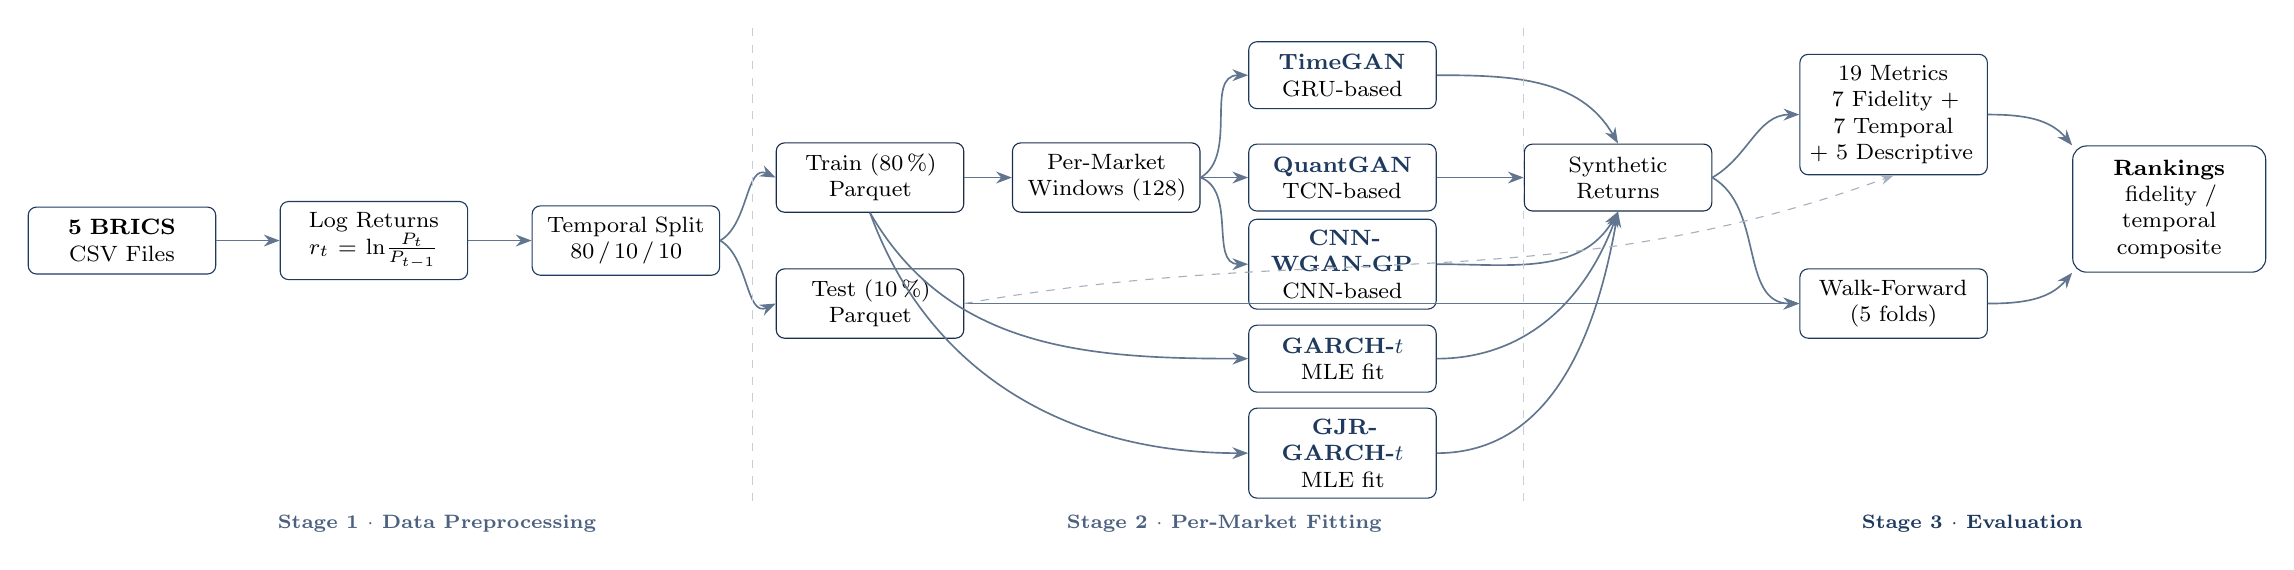
\begin{tikzpicture}[
  every node/.style={font=\footnotesize},
  pp/.style={rectangle, rounded corners=3pt, draw=Navy, fill=LBg,
             text width=2.1cm, align=center, minimum height=0.85cm, inner sep=4pt},
  sp/.style={rectangle, rounded corners=3pt, draw=Sky!80!black, fill=BBg,
             text width=2.1cm, align=center, minimum height=0.85cm, inner sep=4pt},
  ev/.style={rectangle, rounded corners=3pt, draw=Teal, fill=TealBg,
             text width=2.1cm, align=center, minimum height=0.85cm, inner sep=4pt},
  rk/.style={rectangle, rounded corners=5pt, draw=FGreen, fill=GBg,
             text width=2.1cm, align=center, minimum height=1.1cm, inner sep=5pt},
  arr/.style={-Stealth, semithick, draw=Navy!70},
  sarr/.style={-Stealth, thin, draw=Navy!40, dashed},
]
\node[pp] (csv)  at (0.0,  0.0) {\textbf{5 BRICS}\\CSV Files};
\node[pp] (lr)   at (3.2,  0.0) {Log Returns\\$r_t=\ln\!\tfrac{P_t}{P_{t-1}}$};
\node[pp] (spl)  at (6.4,  0.0) {Temporal Split\\80\,/\,10\,/\,10};
\node[sp] (trn)  at (9.5,  0.8) {Train (80\,\%)\\Parquet};
\node[sp] (tst)  at (9.5, -0.8) {Test (10\,\%)\\Parquet};
\node[sp] (poo)  at (12.5,  0.8) {Per-Market\\Windows (128)};
\node[rectangle,rounded corners=3pt,draw=TGcol,fill=ABg,
      text width=2.1cm,align=center,minimum height=0.85cm,inner sep=4pt]
     (tga) at (15.5,  2.1) {\textcolor{TGcol}{\bfseries TimeGAN}\\GRU-based};
\node[rectangle,rounded corners=3pt,draw=QGcol,fill=BBg,
      text width=2.1cm,align=center,minimum height=0.85cm,inner sep=4pt]
     (qga) at (15.5,  0.8) {\textcolor{QGcol}{\bfseries QuantGAN}\\TCN-based};
\node[rectangle,rounded corners=3pt,draw=FGcol,fill=GBg,
      text width=2.1cm,align=center,minimum height=0.85cm,inner sep=4pt]
     (fga) at (15.5, -0.3) {\textcolor{FGcol}{\bfseries CNN-WGAN-GP}\\CNN-based};
\node[rectangle,rounded corners=3pt,draw=Purple,fill=LBg,
      text width=2.1cm,align=center,minimum height=0.85cm,inner sep=4pt]
     (gar) at (15.5, -1.5) {\textcolor{Purple}{\bfseries GARCH-$t$}\\MLE fit};
\node[rectangle,rounded corners=3pt,draw=Indigo,fill=IBg,
      text width=2.1cm,align=center,minimum height=0.85cm,inner sep=4pt]
     (gjr) at (15.5, -2.7) {\textcolor{Indigo}{\bfseries GJR-GARCH-$t$}\\MLE fit};
\node[sp] (syn)  at (19.0,  0.8) {Synthetic\\Returns};
\node[ev] (sfm)  at (22.5,  1.6) {19 Metrics\\7 Fidelity + 7 Temporal\\+ 5 Descriptive};
\node[ev] (wfv)  at (22.5, -0.8) {Walk-Forward\\(5 folds)};
\node[rk] (rnk)  at (26.0,  0.4) {\textbf{Rankings}\\fidelity / temporal\\composite};
\draw[arr] (csv.east) -- (lr.west);
\draw[arr] (lr.east)  -- (spl.west);
\draw[arr] (spl.east) to[out= 30,in=155] (trn.west);
\draw[arr] (spl.east) to[out=-30,in=205] (tst.west);
\draw[arr] (trn.east) -- (poo.west);
\draw[arr] (poo.east) to[out= 30,in=180] (tga.west);
\draw[arr] (poo.east) --                 (qga.west);
\draw[arr] (poo.east) to[out=-20,in=180] (fga.west);
%% The econometric arm is fed from the raw training returns, not the
%% normalised 128-step windows: the tanh squash would compress exactly the
%% variance dynamics GARCH exists to model (Section~\ref{sec:decisions}).
\draw[arr] (trn.south) to[out=-60,in=180] (gar.west);
\draw[arr] (trn.south) to[out=-70,in=180] (gjr.west);
\draw[arr] (tga.east) to[out=  0,in=120] (syn.north);
\draw[arr] (qga.east) --                 (syn.west);
\draw[arr] (fga.east) to[out=  0,in=240] (syn.south);
\draw[arr] (gar.east) to[out=  0,in=250] (syn.south);
\draw[arr] (gjr.east) to[out=  0,in=260] (syn.south);
\draw[arr]  (syn.east) to[out= 30,in=180] (sfm.west);
\draw[arr]  (syn.east) to[out=-30,in=180] (wfv.west);
\draw[arr]  (tst.east) --                 (wfv.west);
\draw[sarr] (tst.east) to[out=10,in=200]  (sfm.south);
\draw[arr] (sfm.east) to[out=0,in=130] (rnk.north west);
\draw[arr] (wfv.east) to[out=0,in=230] (rnk.south west);
\node[font=\scriptsize\bfseries,text=Navy!80]  at ( 4.0,-3.6) {Stage 1 $\cdot$ Data Preprocessing};
\node[font=\scriptsize\bfseries,text=Navy!80]  at (14.0,-3.6) {Stage 2 $\cdot$ Per-Market Fitting};
\node[font=\scriptsize\bfseries,text=Teal]     at (23.5,-3.6) {Stage 3 $\cdot$ Evaluation};
\draw[very thin,dashed,Navy!25] ( 8.0, 2.7) -- ( 8.0,-3.4);
\draw[very thin,dashed,Navy!25] (17.8, 2.7) -- (17.8,-3.4);
\end{tikzpicture}
}
\caption{The pipeline. Data are prepared once; every model is then fitted independently per market and seed, evaluated against the real test series and in walk-forward folds, and ranked.}
\label{fig:pipeline}
\end{figure}
\end{landscape}

\subsection{Data preparation}
Closing prices are read with an explicit date format and sorted chronologically before anything else is computed; daily log returns are $r_t=\ln(P_t/P_{t-1})$, with no clipping of outliers. Each market's series is split in time into training, validation and test parts (80/10/10) and stored as Parquet files. For the gradient-trained models the training part is cut into overlapping windows of 128 returns with stride 1.

\subsection{Training with budget parity}
Every model is trained or fitted independently for each market and each seed (42, 43, 44), on that market's training split only. The three GANs standardise returns and squash them with $\tanh(z/3)$, and train for exactly 9,000 generator updates; the pipeline asserts that the three budgets are equal and refuses to run otherwise. TimeGAN first runs its autoencoder and supervisor pre-training. The two econometric models are fitted by maximum likelihood on returns scaled by 100, in two stages: an unconstrained fit whose persistence is always recorded, and a refit under a stationarity bound only when that persistence reaches 1 (Section~\ref{sec:boundary}). Weights and fitted parameters are saved for every production model.

\subsection{Walk-forward validation}
Walk-forward validation re-runs training on growing windows of the full series. With $n$ observations and $K=5$ folds, each test block has $L=\lfloor n/(K+1)\rfloor$ observations; fold $k$ trains a fresh model on the first $n-L(K-k)$ observations and generates a series the length of the following block. Training data therefore always precede test data, and later folds train on more history. Each fold records Wasserstein and energy distance, quantile MSE, the Hurst and ARCH-LM differences and discriminative AUC.

\subsection{Evaluation}
Each fitted model generates one series with as many observations as the market's real test split. Every metric in Table~\ref{tab:metrics} compares it with the real test series. A shuffled control --- a fixed random permutation of the same real test series --- is scored by the same code. For downstream utility each model's per-market draws are saved, then concatenated across all markets for each seed, and a single variance-forecasting backtest is run on the pooled sample.

\subsection{Ranking}
Within each market--seed evaluation, the five generators are ranked on every ranked metric; the control is excluded, and a metric that cannot be computed ranks last. Fidelity and temporal ranks are the means within each family and the composite rank is their mean. Ranks are then averaged over all 15 evaluations.

\subsection{Reporting}
Per-market results are written to disk as each evaluation completes, and aggregates are read back from disk rather than from memory, so an interrupted run resumes without losing completed work; a completed evaluation is skipped only if its recorded configuration --- budgets, folds, model roster and code version --- matches the run about to start. This report is built by \texttt{generate\_report.py} from those files through \texttt{report\_data.py}, which raises rather than substituting a value when an artifact is missing. A regression check, \texttt{verify\_notebook.py}, guards the pipeline's safeguards before every commit.
%% ─── Results ─────────────────────────────────────────────────────────────────
\section{Results}
\label{sec:results}
All tables pool 15 evaluations: 5 markets $\times$ 3 seeds. The figures show one of them, BOVESPA with seed 42, as an illustration of what the metrics measure; the rankings rest on the tables, not on the figures.

%% ── Ranking ──
\subsection{Overall ranking}
\label{sec:ranking}

\begin{table}[htbp]
\centering
\caption{Mean ranks over 15 market--seed evaluations; lower is better. \emph{Wins}: evaluations in which the model has the lowest composite rank. \emph{Fit}: mean wall-clock seconds to train or fit one model. The shuffled control is scored on every metric but does not compete for rank.}
\label{tab:ranking}
\begin{tabular}{@{}llccccr@{}}
\toprule
Model & Family & Composite & Fidelity & Temporal & Wins & Fit (s) \\
\midrule
GJR-GARCH & econometric & \textbf{2.524} & 2.667 & 2.381 & 2\,/\,15 & $<1$ \\
CNN-WGAN-GP & gradient & 2.605 & 2.429 & 2.781 & 6\,/\,15 & 180 \\
GARCH & econometric & 2.967 & 3.152 & 2.781 & 3\,/\,15 & $<1$ \\
QuantGAN & gradient & 3.041 & 3.138 & 2.943 & 2\,/\,15 & 481 \\
TimeGAN & gradient & 3.864 & 3.614 & 4.114 & 2\,/\,15 & 81 \\
\bottomrule
\end{tabular}
\end{table}

\paragraph{What it shows} Table~\ref{tab:ranking} gives, for each generator, its mean rank on the two metric families and on their combination, and how often it wins an evaluation outright.

\paragraph{How it is computed} Within each evaluation the five generators are ranked on each of the fourteen ranked metrics of Table~\ref{tab:metrics}, rank~1 being closest to the real series. The fidelity rank is the mean over the seven fidelity metrics, the temporal rank the mean over the seven temporal metrics, and the composite rank the mean of the two, so the two families weigh equally however many metrics each contains. The ranks are then averaged over the evaluations.

\paragraph{Why this measure} Ranks rather than raw values, because the metrics live on incommensurable scales. The equal weighting of families is this study's own design, adopted because an unweighted mean over all metrics is won by a shuffled copy of the data (Section~\ref{sec:families}).

\paragraph{What this result tells us} GJR-GARCH has the best mean composite rank (2.524); CNN-WGAN-GP trails by 0.081 (2.605). The families split along the metric families: CNN-WGAN-GP leads on fidelity, the marginal distribution, and GJR-GARCH on temporal, the dynamics. Counted per evaluation the picture runs the other way from the mean. Composite wins are CNN-WGAN-GP 6, GARCH 3, GJR-GARCH 2, QuantGAN 2, TimeGAN 2 --- the gradient-trained family takes 10 of 15 and the econometric family 5; temporal wins are GJR-GARCH 6, GARCH 3, CNN-WGAN-GP 2, QuantGAN 2, TimeGAN 2; fidelity wins are CNN-WGAN-GP 5, GARCH 3, GJR-GARCH 3, QuantGAN 3, TimeGAN 1. The econometric advantage is therefore in the mean rank and in the dynamics, not in winning most individual evaluations. An unweighted mean over all ranked metrics is kept in the artifacts for comparability and is never used for selection.

%% ── Compute ──
\subsection{Compute versus performance}
\label{sec:compute}
Table~\ref{tab:compute}, in Section~\ref{sec:architecture}, sets each model's size and training cost against its composite rank --- the one comparison a rank column cannot make. Parameter counts are read from the fitted models and wall-clock is measured around training or fitting. The best-ranked model, GJR-GARCH, has 6 parameters and fits in 0.018\,s. The largest, QuantGAN, has 276,481 --- a factor of 46,080 --- and takes 481\,s, a factor of 27,184; it ranks below the smaller model on composite, on fidelity and on temporal.

The ratio is stated and left there. It does not show that parameter count is wasted in general, that the generators would not overtake the baselines at a larger budget, or that they are at their best configuration: no hyperparameter search was run (Section~\ref{sec:limitations}). What it shows is that on these data, at this budget, under this evaluation, the additional capacity did not buy additional rank.

%% ── Figures ──
\subsection{Stylised facts in the generated series}
\label{sec:stylised}
The figures in this section are crops of one figure drawn by the pipeline for BOVESPA, seed 42, set at full page width so their labels can be read. Each shows a single generated series per model: they show what the metrics measure, and the numbers that rank the models are in the tables.

\subsubsection{The generated series}
\label{sec:series}

\begin{landscape}
\begin{figure}[p]
\centering

\includegraphics[width=\linewidth,trim=0.00 1618.08 0.00 22.80,clip]{thesis_results/production/BOVESPA/seed42/BOVESPA_stylized_facts.png}
\caption{One generated series per model beside the real test series, BOVESPA, seed 42: the real series and the three GANs (continued in Figure~\ref{fig:series-b}). All rows share one vertical scale, in daily log return. The horizontal axis is a common index of trading days, not common calendar time: real and synthetic series are independent draws, so vertical alignment between rows carries no meaning.}
\label{fig:series-a}
\end{figure}
\end{landscape}

\begin{landscape}
\begin{figure}[p]
\centering

\includegraphics[width=\linewidth,trim=0.00 1146.48 0.00 618.72,clip]{thesis_results/production/BOVESPA/seed42/BOVESPA_stylized_facts.png}
\caption{Continuation of Figure~\ref{fig:series-a}: the two GARCH baselines and the shuffled control --- the real test series in random order --- on the same vertical scale.}
\label{fig:series-b}
\end{figure}
\end{landscape}

\paragraph{What they show} Figures~\ref{fig:series-a} and~\ref{fig:series-b} plot a synthetic series from each fitted model, the real test series, and the shuffled control.

\paragraph{How they are computed} Each model, fitted on the market's training split, generates one series with as many observations as the real test split. The control is a random permutation of the real test series. Nothing is smoothed or rescaled.

\paragraph{Why this view} Volatility clustering --- large moves arriving in bursts rather than evenly scattered --- is the stylised fact visible to the eye (Mandelbrot\tcite{9}; Cont\tcite{7}). The shuffled control is the reference for its absence: it contains exactly the real values, in random order.

\paragraph{What this example tells us} One draw is an illustration, not a statistic. Read with that caveat, the panels show why models can look plausible and still score differently: in this example the TimeGAN path oscillates with an unusually regular pattern, and the QuantGAN path concentrates its largest moves in a single burst. The mode-collapse guard of Section~\ref{sec:collapse}, which flags a high lag-1 autocorrelation, is the quantitative counterpart of a visibly regular path.

\subsubsection{Marginal distribution: the Q--Q plot}
\label{sec:qq}

\begin{figure}[htbp]
\centering

\includegraphics[width=\linewidth,trim=0.00 887.04 569.52 1090.32,clip]{thesis_results/production/BOVESPA/seed42/BOVESPA_stylized_facts.png}
\caption{Quantiles of each synthetic series against the same quantiles of the real series, at 200 probability levels from 0.5\% to 99.5\%. The black diagonal is a perfect match. The inset lists each series' two-sample Kolmogorov--Smirnov statistic, drawn for orientation only.}
\label{fig:qq}
\end{figure}

\paragraph{What it shows} Figure~\ref{fig:qq} compares each model's distribution of daily returns with the real one, quantile by quantile.

\paragraph{How it is computed} For each probability $p$ from 0.005 to 0.995, the $p$-quantile of the synthetic series is plotted against the $p$-quantile of the real series. Identical distributions put every point on the diagonal. A curve steeper than the diagonal in a tail means the model's tail is wider than the real one; a flatter curve means it is narrower.

\paragraph{Why this measure} The Q--Q plot\tcite{44} compares whole distributions without binning and shows the tails, where risk sits, at the same resolution as the centre. Its ranked counterparts are \texttt{quantile\_mse} and \texttt{wasserstein} (Table~\ref{tab:metrics}).

\paragraph{What this example tells us} The shuffled control lies on the diagonal by construction, because it is the real data reordered. That is exactly why a Q--Q plot, like every fidelity metric, cannot on its own tell a good generator from a shuffled deck. The differences are in the tails: here the QuantGAN curve bends far below the diagonal in the lower tail, generating losses several times larger than the real series' worst days, while the TimeGAN curve flattens and compresses both tails.

\subsubsection{Tails: the survival function on log--log axes}
\label{sec:survival}

\begin{figure}[htbp]
\centering

\includegraphics[width=\linewidth,trim=582.48 887.04 0.00 1090.32,clip]{thesis_results/production/BOVESPA/seed42/BOVESPA_stylized_facts.png}
\caption{Empirical survival function $P(|r|>x)$ of each series on log--log axes. A power-law tail $P(|r|>x)\propto x^{-\alpha}$ is a straight line on these axes, and its slope is $-\alpha$, the tail index. Lines stop at roughly $1/n$, where a single observation fixes the estimate.}
\label{fig:survival}
\end{figure}

\paragraph{What it shows} Figure~\ref{fig:survival} shows how quickly the probability of a move larger than $x$ decays as $x$ grows.

\paragraph{How it is computed} For each series, absolute returns are sorted and each value $x$ is plotted against the fraction of observations that exceed it. The largest one per cent of order statistics is left off the drawn line, because each is a single-observation estimate of a very small probability; no metric is affected by this.

\paragraph{Why this measure} Tails that decay like a power law are the first stylised fact of returns (Mandelbrot\tcite{9}; Cont\tcite{7}). The log--log survival plot is how that exponent is seen, and the Hill estimator\tcite{38} is how it is measured: \texttt{tail\_index\_diff} ranks models by the gap between the real and synthetic Hill estimates (Section~\ref{sec:tail}).

\paragraph{What this example tells us} A line parallel to the real one has the right tail index; a line that drops away early under-produces extremes; a line that extends to the right produces moves larger than any in the real data. Here the QuantGAN line extends several times beyond the real series' largest absolute return --- the same excess the Q--Q plot shows --- while the two GARCH lines stay close to the real one.

\subsubsection{Autocorrelation of returns, absolute returns and squared returns}
\label{sec:acf}

\begin{figure}[htbp]
\centering

\includegraphics[width=\linewidth,trim=0.00 628.32 566.16 1349.76,clip]{thesis_results/production/BOVESPA/seed42/BOVESPA_stylized_facts.png}\\[6pt]

\includegraphics[width=\linewidth,trim=585.84 628.32 0.00 1349.76,clip]{thesis_results/production/BOVESPA/seed42/BOVESPA_stylized_facts.png}\\[6pt]

\includegraphics[width=\linewidth,trim=0.00 369.60 575.52 1608.48,clip]{thesis_results/production/BOVESPA/seed42/BOVESPA_stylized_facts.png}
\caption{Sample autocorrelation of returns (top), absolute returns (middle) and squared returns (bottom) at lags 0 to 50. Red dotted lines mark $\pm1.96/\sqrt{n}$, the approximate 95\% band for a series with no autocorrelation. The MAE values annotated in one panel average lags 1 to 20, not the window of the ranked metric (see text).}
\label{fig:acf}
\end{figure}

\paragraph{What they show} Figure~\ref{fig:acf} shows how strongly each series is correlated with its own past, separately for the direction of moves ($r_t$) and for their size ($|r_t|$ and $r_t^2$).

\paragraph{How they are computed} At lag $k$, $\hat\rho(k)=\sum_t(x_t-\bar x)(x_{t+k}-\bar x)\big/\sum_t(x_t-\bar x)^2$, with $x_t$ equal to $r_t$, $|r_t|$ or $r_t^2$. The ranked metrics \texttt{acf\_returns\_mae}, \texttt{acf\_absolute\_mae} and \texttt{acf\_squared\_mae} are the mean absolute difference between the real and synthetic $\hat\rho(k)$ over lags 1 to $\min(50,\lfloor n/4\rfloor)$, which is 50 at the test-series lengths used here.

\paragraph{Why this measure} Returns themselves are close to uncorrelated, while their absolute and squared values stay positively autocorrelated for many lags. That is volatility clustering (Cont\tcite{7}; Ding, Granger \& Engle\tcite{8}), the regularity ARCH and GARCH models were built to describe (Engle\tcite{10}; Bollerslev\tcite{39}). A generator that matches the distribution of returns but not these curves has not learned the dynamics.

\paragraph{What this example tells us} In this test window the real series' autocorrelation of squared returns stays close to the no-autocorrelation band, so clustering in the real data is weak here, while the QuantGAN and TimeGAN curves sit well above it at short lags: these generators produce more persistent volatility than the data. Section~\ref{sec:audit} gives the pooled numbers: on \texttt{acf\_squared\_mae} a shuffled copy of the real series beats all 3 GANs.

\paragraph{A discrepancy, reported rather than changed} The MAE values annotated in the figure average lags 1 to 20 and describe themselves as matching the ranked metric. The ranked metric, as the pipeline computes it at these series lengths, averages lags 1 to 50. The ranked values in this report are the pipeline's. Which window was intended is a question about the metric's definition, and it has not been changed here.

\subsubsection{Rolling volatility}
\label{sec:rolling}

\begin{figure}[htbp]
\centering

\includegraphics[width=\linewidth,trim=576.48 369.60 0.00 1608.48,clip]{thesis_results/production/BOVESPA/seed42/BOVESPA_stylized_facts.png}
\caption{Twenty-day rolling standard deviation of each series over its first 500 observations. The horizontal axis is an index, not calendar time.}
\label{fig:rolling}
\end{figure}

\paragraph{What it shows} Figure~\ref{fig:rolling} shows how the local scale of each series changes over time.

\paragraph{How it is computed} The standard deviation of the preceding 20 daily log returns, recomputed each day, over the first 500 days of each series.

\paragraph{Why this measure} Rolling volatility makes clustering visible as slow swings between calm and turbulent periods --- the behaviour conditional-variance models describe (Engle\tcite{10}; Bollerslev\tcite{39}). It is a visual check rather than a ranked metric; its quantitative counterparts are the autocorrelation metrics above and \texttt{hurst\_diff}.

\paragraph{How to read it} A line that stays flat has no clustering. A line with a single tall spike concentrates its turbulence in one episode. A line whose swings resemble the real one in both height and duration reproduces the clustering the metrics look for.

\subsubsection{Moments}
\label{sec:moments}

\begin{figure}[htbp]
\centering

\includegraphics[width=\linewidth,trim=0.00 126.96 565.68 1867.20,clip]{thesis_results/production/BOVESPA/seed42/BOVESPA_stylized_facts.png}\\[6pt]

\includegraphics[width=\linewidth,trim=586.32 126.96 0.00 1867.20,clip]{thesis_results/production/BOVESPA/seed42/BOVESPA_stylized_facts.png}
\caption{Sample moments of each series: mean and standard deviation (top), skewness and excess kurtosis (bottom). The shape moments are descriptive only.}
\label{fig:moments}
\end{figure}

\paragraph{What it shows} Figure~\ref{fig:moments} shows the first four sample moments of each series beside those of the real test series.

\paragraph{How it is computed} The mean, standard deviation, skewness and excess kurtosis of each series' daily log returns.

\paragraph{Why this measure} Location and scale are ranked, through \texttt{mean\_diff} and \texttt{std\_diff}. Skewness and kurtosis are shown but never ranked. With tail index $\alpha$, the moment $\E|r|^k$ exists only for $k<\alpha$ (Hill\tcite{38}); at the tail indices of these markets population kurtosis does not exist, so its sample value grows with the sample instead of converging (Section~\ref{sec:decisions}).

\paragraph{What this example tells us} Excess kurtosis differs by an order of magnitude between models --- the QuantGAN bar stands far above the real one. That is exactly the kind of difference that looks decisive and is not: with no finite population kurtosis to estimate, a larger sample could move it arbitrarily far.

%% ── Audit ──
\subsection{The shuffled-control audit}
\label{sec:audit}

\paragraph{Permutation invariance, counted} The control is the pooled real test series in random order (\texttt{numpy.random.default\_rng(42).permutation}). It has the identical marginal distribution --- same values, same histogram, same moments, same tails --- and no temporal structure whatsoever. It is useless for every application synthetic market data is generated for, and it is scored by the full pipeline alongside every generator.

A metric is counted as permutation-invariant in practice when the control's mean value is negligible against the best real generator's on the same metric. On this run that criterion separates cleanly: every metric it selects has a ratio below 3.6e-05, and the smallest ratio among the metrics it does not select is 0.36. There is nothing in the gap, so the cut is not a judgement call.

\textbf{9 of 19} computed metrics are permutation-invariant:
{\footnotesize\texttt{mean\_diff, std\_diff, skewness\_diff, kurtosis\_diff, wasserstein, energy\_distance, quantile\_mse, tail\_index\_diff, extreme\_events\_diff}}

Under an unweighted mean over all metrics, the control ranks first --- the finding that produced the two-family composite. That is a structural property of any metric defined on the marginal distribution alone, not a quirk of these choices: mean, variance, kurtosis, Wasserstein distance and energy distance all belong to that class. Any evaluation of synthetic financial data built only from distributional metrics cannot distinguish a working generator from a shuffled deck.

\begin{table}[htbp]
\centering
\caption{The shuffled control against the generators on four ordering-sensitive metrics: means over 15 evaluations, lower is better. The control's value and every generator that beats it are set in bold.}
\label{tab:control}
\begin{tabular}{@{}lcccccc@{}}
\toprule
Metric & Control & CNN-WGAN-GP & GARCH & GJR-GARCH & QuantGAN & TimeGAN \\
\midrule
ACF$(r)$ MAE & \textbf{0.0517} & \textbf{0.0511} & 0.0517 & \textbf{0.0514} & 0.0548 & 0.0685 \\
ACF$(r^2)$ MAE & \textbf{0.0570} & 0.0590 & 0.0574 & \textbf{0.0544} & 0.0806 & 0.1002 \\
ACF$(|r|)$ MAE & \textbf{0.0730} & \textbf{0.0610} & \textbf{0.0627} & \textbf{0.0610} & 0.0981 & 0.1232 \\
Hurst diff & \textbf{0.0759} & \textbf{0.0369} & \textbf{0.0397} & \textbf{0.0341} & \textbf{0.0400} & 0.0881 \\
\bottomrule
\end{tabular}
\end{table}

\paragraph{What it shows} Table~\ref{tab:control} compares the control with each generator on the four metrics a shuffled series should fail: the autocorrelation of returns, of absolute returns and of squared returns, and long memory.

\paragraph{How it is computed} Each value is the metric's mean over all evaluations. The control is scored by exactly the code that scores the generators.

\paragraph{Why this measure} These metrics are ordering-sensitive by construction --- they measure volatility clustering (Cont\tcite{7}; Ding, Granger \& Engle\tcite{8}) and long memory (Hurst\tcite{23}) --- so a series with no dynamics should lose to any generator that has learned some.

\paragraph{What this result tells us} On the autocorrelation of squared returns, the canonical volatility-clustering statistic, the shuffled control beats all 3 GANs, and CNN-WGAN-GP, GARCH, QuantGAN, TimeGAN in all; only GJR-GARCH clears it. On absolute returns the control beats QuantGAN, TimeGAN, and CNN-WGAN-GP, GARCH, GJR-GARCH clear it. On returns it beats GARCH, QuantGAN, TimeGAN, and the models that clear it do so by only 0.0003 to 0.0006. On the Hurst difference it beats TimeGAN alone. A shuffled copy of the real series, with no temporal information at all, outperforms state-of-the-art GAN architectures on the metrics those architectures exist to satisfy.

\paragraph{What this does and does not license} It is tempting to conclude that these ACF metrics are ``really'' permutation-invariant too, and to move the headline count from 9 to a larger number. We do not, and the reason is the contribution.

\textbf{These metrics are not permutation-invariant.} They are functions of the ordering, and on every row of Table~\ref{tab:control} at least one model clears the control --- as few as 1 of 5 on ACF$(r^2)$ MAE. A metric that can make that separation is measuring temporal structure. It is doing its job.

\textbf{What fails is the comparison, not the metric.} A metric that separates some models from a shuffled deck and not others is telling us about the models it fails to separate, not about itself. Read the other way round, it is weak evidence about the metric.

\textbf{Therefore: permutation-invariance in practice is a property of the comparison set, not of a metric in isolation.} The same metric is discriminating against one model and uninformative against another, in the same run, on the same data. A count of ``how many metrics are permutation-invariant'' is only meaningful once the set of models being compared is fixed --- and reporting one without the other is how a suite comes to look more discriminating than it is.

We keep the headline at 9 of 19: the metrics that are invariant by construction. The ACF results are reported as what they are: 4 of the 5 generators lose to the control on at least one ordering-sensitive metric, on the metrics most often used to claim success --- and \texttt{FIDELITY\_COLS} and \texttt{TEMPORAL\_COLS} are unchanged.

The practical recommendation follows: a shuffled control belongs in every evaluation table for synthetic time series, permanently, in the role a positive control plays in a biology experiment. It costs one permutation and it is the only line in the table that cannot be gamed by learning the marginal.

%% ── Walk-forward ──
\subsection{Walk-forward discriminability}
\label{sec:walkforward}

\begin{table}[htbp]
\centering
\caption{Discriminative AUC over every walk-forward fold of every evaluation. $|\mathrm{AUC}-0.5|$ is the ranked quantity; $z$ is the distance of the mean AUC from the empirical null of $0.506\pm0.084$, in null standard deviations.}
\label{tab:auc}
\begin{tabular}{@{}lcccr@{}}
\toprule
Model & AUC (mean $\pm$ sd) & $|\mathrm{AUC}-0.5|$ & $z$ vs null & Folds \\
\midrule
CNN-WGAN-GP & 0.637 $\pm$ 0.136 & 0.137 & 1.56 & 75 \\
GARCH & 0.683 $\pm$ 0.167 & 0.183 & 2.10 & 75 \\
GJR-GARCH & 0.655 $\pm$ 0.164 & 0.155 & 1.78 & 75 \\
QuantGAN & 0.741 $\pm$ 0.175 & 0.241 & 2.80 & 75 \\
TimeGAN & 0.814 $\pm$ 0.144 & 0.314 & 3.66 & 75 \\
\bottomrule
\end{tabular}
\end{table}

\begin{table}[htbp]
\centering
\caption{Mean discriminative AUC by walk-forward fold, over all models and markets. The training window grows with the fold.}
\label{tab:folds}
\begin{tabular}{@{}lccc@{}}
\toprule
Fold & Training length & Mean AUC & sd \\
\midrule
0 & 810--837 & 0.811 & 0.154 \\
1 & 1,620--1,669 & 0.692 & 0.135 \\
2 & 2,430--2,501 & 0.747 & 0.147 \\
3 & 3,240--3,333 & 0.616 & 0.177 \\
4 & 4,050--4,165 & 0.664 & 0.166 \\
\bottomrule
\end{tabular}
\end{table}

\paragraph{What they show} Tables~\ref{tab:auc} and~\ref{tab:folds} show whether a classifier can tell each model's output from real data out of sample, and how that changes as the training window grows.

\paragraph{How they are computed} In each of the 5 walk-forward folds (Section~\ref{sec:pipeline}) a freshly trained model generates a series the length of the fold's test block. A logistic regression then tries to separate real from synthetic 20-day windows described by their mean, standard deviation, mean absolute return and mean squared return, scored by five-fold cross-validation without shuffling. An AUC of 0.5 means the two are indistinguishable.

\paragraph{Why this measure} A classifier-based discriminative score is the indistinguishability test of TimeGAN\tcite{4}, adopted by CTBench\tcite{16}. Walk-forward evaluation keeps test data strictly after training data, as time-series evaluation requires (Tashman\tcite{13}; Bergmeir \& Ben\'{\i}tez\tcite{14}). The null is not exactly 0.5: over 15 real-versus-real half-splits it was $0.506\pm0.084$, a prior measurement, so each AUC is read as a distance from that null.

\paragraph{What this result tells us} 3 of 5 models sit more than 1.96 null standard deviations from it (TimeGAN, QuantGAN, GARCH). The rest (CNN-WGAN-GP, GJR-GARCH) lie within that distance on the fold-averaged mean, so on this metric alone they cannot be distinguished from a perfect generator at the 5\% level; 5 of 5 mean AUCs lie above the null mean. AUC falls as the training window grows, from 0.811 at fold 0 (training on 810--837 observations) to 0.664 at fold 4 (4,050--4,165), but the decline is not monotonic: fold(s) 2, 4 rise above the fold before. Fold index, training length and the calendar period a fold covers all advance together, so this design cannot separate ``more training data helps'' from ``the later period is easier to imitate''.

%% ── Tail index ──
\subsection{Tail index}
\label{sec:tail}

\begin{table}[htbp]
\centering
\caption{\texttt{tail\_index\_diff}, the absolute difference between the real and synthetic Hill tail-index estimates, over all evaluations.}
\label{tab:tail}
\begin{tabular}{@{}lccc@{}}
\toprule
Model & Mean & sd & Observed range \\
\midrule
CNN-WGAN-GP & 0.943 & 0.831 & 0.208--2.871 \\
GARCH & 1.195 & 1.062 & 0.086--3.785 \\
GJR-GARCH & 1.316 & 0.856 & 0.019--2.385 \\
QuantGAN & 1.079 & 0.892 & 0.146--3.211 \\
TimeGAN & 2.682 & 3.330 & 0.024--9.825 \\
\bottomrule
\end{tabular}
\end{table}

\paragraph{What it shows} Table~\ref{tab:tail} shows how far each model's tail heaviness is from the real series', and how much that varies across evaluations.

\paragraph{How it is computed} The Hill estimator\tcite{38} takes the absolute returns above their 95th percentile $u$, $X_1,\dots,X_k$, and estimates the tail index as $\hat\alpha=\big[\frac1k\sum_i\log(X_i/u)\big]^{-1}$; an estimate above 20 means the series has effectively no tail and counts as a failure. The metric is $|\hat\alpha-\tilde{\hat\alpha}|$.

\paragraph{What this result tells us} TimeGAN sits at 2.68 against 0.94--1.32 for the other four --- a real and large gap. But the dispersion swamps the comparison between the rest: the spread between model means is 1.74, and the largest standard deviation within one model is 3.33, which exceeds it. Market-to-market and run-to-run variation on this metric is larger than most differences between models, so a single-run winner on \texttt{tail\_index\_diff} is not a finding, and none is reported.

%% ── Mode collapse ──
\subsection{Mode collapse}
\label{sec:collapse}
The pipeline's post-generation guard checks every generated series and prints a \texttt{[WARNING]} when the lag-1 autocorrelation exceeds $|0.1|$ --- a return series should have almost none, and a high value means a smooth path rather than returns.

In this run the guard fired \textbf{18 times}, across 2 model(s) --- TimeGAN (16), QuantGAN (2). Mean \(|\text{ACF}(1)| = 0.533\), over the range \(-0.622\) to \(0.942\); generated sd 0.0002--0.0440. Read from \texttt{run\_log\_20260912\_131816.log}.

The ranking agrees. TimeGAN is the worst of the five on \textbf{all 7 of 7 temporal metrics}, on 5 of 7 fidelity metrics, and on 14 of the 19 computed metrics overall. It is \emph{not} worst on std\_diff (QuantGAN), skewness\_diff (QuantGAN), quantile\_mse (QuantGAN), arch\_pvalue\_diff (GARCH), arch\_stat\_diff (QuantGAN) --- the model in brackets is worse there --- so ``worst on every metric'' would be an overstatement, and the scope is stated instead.

\textbf{An earlier explanation is withdrawn.} A previous draft attributed this to tanh saturation in the Recovery network. This run's own \texttt{[DIAG]} latent instrumentation does not support that: across 90 latent readings saturation never exceeds 3.1\% against the 50\% threshold the diagnostic exists to detect, and across 90 reconstruction readings output sd never differs from target sd by more than 0.0014, so the autoencoder is functioning. The collapse is real and the mechanism is open.

%% ── Boundary ──
\subsection{GARCH fits at the integrated boundary}
\label{sec:boundary}

\paragraph{What it shows} How often a GARCH or GJR-GARCH fit converged to a persistence of 1 --- the point at which the conditional variance never reverts to a long-run level --- and what the pipeline did about it.

\paragraph{How it is computed} Persistence is $\alpha+\beta$ for GARCH(1,1)\tcite{39} and $\alpha+\beta+\gamma/2$ for GJR-GARCH(1,1)\tcite{40}, \texttt{arch}'s own definition. Every econometric fit --- the main fit and one fit per walk-forward fold, for both models --- records its unconstrained persistence. A fit within $10^{-6}$ of 1 is refitted under the bound persistence $\le 1-10^{-4}$, and its output is generated from the constrained parameters.

\paragraph{Boundary fits, counted} Every econometric fit records its unconstrained persistence as a result: the main fit on each training split and one per walk-forward fold, for both GARCH variants. Across 180 fits (60 market--window--model combinations $\times$ 3 seeds; a fit does not depend on the seed), \textbf{12 reached the integrated boundary} --- persistence within $10^{-6}$ of 1 --- in 4 combinations, on NIFTY50, SHANGHAI. The constraint was applied to exactly those fits and to no other.

\smallskip
{\footnotesize
\begin{tabular}{@{}lllrrc@{}}
\toprule
Market & Window & Model & Unconstrained & Constrained & Seeds \\
\midrule
NIFTY50 & fold 0 & GARCH & 1.0000000000 & 0.9999000000 & 3 \\
SHANGHAI & main & GARCH & 1.0000000000 & 0.9999000000 & 3 \\
SHANGHAI & fold 3 & GARCH & 1.0000000000 & 0.9999000000 & 3 \\
SHANGHAI & fold 3 & GJR-GARCH & 1.0000000000 & 0.9999000000 & 3 \\
\bottomrule
\end{tabular}}

\smallskip
Boundary fits sit within $3.5\times10^{-13}$ of 1; the largest persistence among the other 168 fits is 0.99987666 ($1-p$ = $1.23\times10^{-4}$). Constrained persistence is 0.9999000000--0.9999000000, at a log-likelihood change of -0.019743 to -0.000581 --- the constrained fit is statistically indistinguishable from the unconstrained one, which is what makes $\delta=10^{-4}$ a calibrated choice rather than an arbitrary one.

\paragraph{The hits are seed-invariant} Each combination above appears in all 3 of 3 seeds, and the log-likelihood cost of the refit is identical across seeds (largest spread 0.000000). A fit by maximum likelihood on fixed data cannot depend on the seed, so this is what should happen --- and it establishes the hits as a property of the data window rather than of estimation noise, which is what licenses reading them as a statement about the data rather than about the estimator.

\paragraph{Two distinct causes} 3 of the affected combinations sit on long windows (3,240--3,888 observations, against a median fitted window of 2,870): SHANGHAI main GARCH; SHANGHAI fold 3 GARCH; SHANGHAI fold 3 GJR-GARCH. These are the structural-break mechanism --- breaks in the unconditional variance absorbed as persistence (Lamoureux \& Lastrapes 1990\tcite{42}; Mikosch \& St\u{a}ric\u{a} 2004\tcite{43}). SHANGHAI over 2006--2026 spans the 2007 bubble and crash, 2015 and COVID: three volatility regimes inside one training window. 1 sits on a short window (829 observations, the shortest walk-forward fold): NIFTY50 fold 0 GARCH. That is a small-sample effect --- at that length the data does not separate slow mean reversion in variance from its absence --- and is reported separately: only the first group is evidence about market structure. At $\alpha+\beta=1$ the conditional variance is a martingale with no unconditional variance to revert to, so simulated paths random-walk without an anchor.

\paragraph{The two-stage fit, and why it is done at fit time} \textbf{Two-stage fit.} Stage~1 fits by maximum likelihood without further constraint and always records persistence ($\alpha+\beta$, plus $\gamma/2$ for GJR-GARCH --- \texttt{arch}'s own definition). Stage~2 runs only when stage~1 lands within $10^{-6}$ of 1: it refits under persistence $\le 1-\delta$, $\delta=10^{-4}$, and output is generated from the constrained parameters; both parameter sets are stored with the fit. The refit tightens the right-hand side of \texttt{arch}'s own stationarity constraint and re-optimises \texttt{arch}'s own likelihood, so nothing is reimplemented, and on stationary windows it reproduces the unconstrained fit. $\delta$ sits in an observed gap: across 110 refits, 6 were within $1.7\times10^{-13}$ of 1 and every other fit at least $1.23\times10^{-4}$ below it, so the bound binds only on fits that were already at the boundary.

\smallskip
\textbf{Why at fit time.} Whether a boundary fit explodes is arbitrary. In the preceding run, GARCH exploded on SHANGHAI fold~3 for all three seeds while GJR-GARCH, on the same window, did not; local refits reversed it, 200 of 200 simulated paths against 0 of 200. Rejecting explosive draws after generation would keep whichever draws happened to survive; constraining the fit removes the knife-edge. A post-generation guard still raises if output sd leaves $1/10$--$10\times$ the training sd. It is not guaranteed silent: at persistence 0.9999 one simulated path in 200 per boundary window exceeded $10\times$ in local refits (max $20.8\times$), though the pipeline's seeds stayed within $1.7\times$. The refit counts and the knife-edge are prior measurements recorded in the repository's standing constraints, not artifacts of this run.

\smallskip
\textbf{What it prevented.} In the run that preceded this procedure, the unconstrained fit on the same SHANGHAI fold~3 window generated walk-forward Wasserstein of 74.795, 7.814 and 43.006 across the three seeds --- against a run-wide median of 0.0025 --- with discriminative AUC of exactly 1.000 in all three (a prior measurement; those artifacts are superseded). In this run the largest walk-forward Wasserstein over all 150 econometric folds is 0.01427 against a median of 0.00227, and 0 of them reach AUC 1.000.

%% ── Downstream ──
\subsection{Downstream utility}
\label{sec:downstream}

\begin{table}[htbp]
\centering
\caption{Train on synthetic, test on real: a GARCH(1,1) fitted to each model's synthetic series forecasts the variance of real returns. Medians and means over 3 pooled backtests; lower QLIKE is better. \emph{Fail}: backtests with a degenerate, positive QLIKE.}
\label{tab:downstream}
\begin{tabular}{@{}lrrrrrrc@{}}
\toprule
Model & QLIKE med. & QLIKE mean & Cov.\ err. & Kupiec $p$ & Viol. & $n$ & Fail \\
\midrule
CNN-WGAN-GP & -8.134 & -8.1 & 0.0020 & 0.644 & 129 & 2,479 & --- \\
GJR-GARCH & -8.130 & -8.1 & 0.0068 & 0.110 & 136 & 2,479 & --- \\
QuantGAN & -8.124 & -8.0 & 0.0008 & 0.857 & 122 & 2,479 & --- \\
GARCH & -8.106 & -8.1 & 0.0113 & 0.012 & 138 & 2,479 & --- \\
TimeGAN & -8.102 & -8.0 & 0.0012 & 0.779 & 127 & 2,479 & --- \\
CONTROL: shuffled real & -8.031 & -8.0 & 0.0060 & 0.160 & 109 & 2,479 & --- \\
\bottomrule
\end{tabular}
\end{table}

\paragraph{What it shows} Table~\ref{tab:downstream} asks whether a risk model built on synthetic data works on real data --- the use synthetic market data is wanted for.

\paragraph{How it is computed} For each seed, the real test series of every market are concatenated, and so are each model's per-market synthetic series, in the same order. A Gaussian GARCH(1,1) is fitted to the pooled synthetic series and its parameters are run over the pooled real returns to give one-step variance forecasts $\sigma_t^2$ and a 5\% value-at-risk. QLIKE, $\frac1n\sum_t(\log\sigma_t^2+r_t^2/\sigma_t^2)$, scores the variance forecasts; the Kupiec test checks the rate of VaR violations and the Christoffersen test their independence.

\paragraph{Why this measure} QLIKE is robust to the noise in squared returns as a proxy for variance (Patton\tcite{37}); the Kupiec\tcite{34} and Christoffersen\tcite{35} tests are the standard backtests of a value-at-risk model.

\paragraph{What this result tells us} CNN-WGAN-GP has the lowest median QLIKE ($-$8.134); backtest by backtest, the lowest QLIKE goes to CNN-WGAN-GP 2, GARCH 1. \textbf{Median and mean are both shown.} No model-seed cell returned a positive QLIKE in this run; the largest gap between a model's mean and median QLIKE is 0.125 (TimeGAN).

\paragraph{On $n$} Each backtest runs once per seed over the pooled test set: the real test series of all 5 markets (BOVESPA, FTSE, MOEX, NIFTY50, SHANGHAI) concatenated in market order, with each model's per-market synthetic draws concatenated in the same order. $n$ is 2,479 per backtest, over 3 seeds, so each row above summarises 3 pooled backtests. That $n$ meets the $n\gtrsim600$ at which QLIKE ranks stably, and is close to the $n\approx2{,}480$ at which Kupiec power was measured at $\approx99\%$. Concatenating 5 markets means one GARCH filter crosses 4 market boundaries within 2,479 pooled observations. The shuffled control's QLIKE beats a genuine generator's in 2 of 15 control-versus-generator comparisons (13\%).

\paragraph{ARCH-LM: a regime failure} An 80-replication Monte Carlo (GARCH(1,1), $n=1{,}200$, Gaussian innovations) found \texttt{arch\_pvalue\_diff} identifies the better-fitting model $99\%$ of the time and \texttt{arch\_stat\_diff} $76\%$, the latter with null sd $\approx46.4$ --- two draws from the same process gave LM $56.8$ and $124.8$.

On real BRICS data the pvalue variant saturates completely: real and shuffled series both underflow to $p=0.0$, so $|\Delta p| = 0.000000$ and the metric rates the adversarial control as a perfect match. The stat variant detects the control but is too noisy to rank on.

Neither variant is reliable across both regimes, so both are descriptive-only. ACF-MAE is the primary volatility-clustering ranking signal: continuous, no saturation regime, $88\%$ accuracy in the same Monte Carlo. This is an empirical result about a standard test, not an implementation note.

%% ── Circularity, budget, nondeterminism ──
\subsection{Metric circularity}
\label{sec:circularity}
Stated before a referee states it. \texttt{resid\_kurtosis\_diff} fits a GARCH(1,1) to each series, extracts $\varepsilon_t = r_t/\sigma_t$, and compares the excess kurtosis of those residuals. Two of the five generators \emph{are} GARCH models, so they are being scored, in part, by their own model class.

This is not fatal, and the reason is what the metric asks. It does not ask ``does a GARCH fit this series'' --- that would be circular outright. It asks whether the tails remain heavy \emph{after} GARCH has removed what it can explain, which is Cont's stylized fact 7\tcite{7} and a property a GARCH-$t$ generator can fail. The measured values bear this out: the econometric models score GARCH 3.12, GJR-GARCH 3.04, against 2.64--4.02 for the GANs and 0.94 for the shuffled control --- neither scores better than the shuffled control on it.

It remains an advantage of degree, and it is one reason \texttt{composite\_rank} is reported alongside its two components rather than alone --- \texttt{resid\_kurtosis\_diff} is one of seven temporal metrics, and the temporal result does not rest on it. Gaussian QMLE is used for the fit rather than Student-$t$ precisely to avoid the stronger circularity: a $t$ specification absorbs the excess kurtosis by construction and makes the test uninformative for every model.

\subsection{What the budget choice cost}
\label{sec:budget}
Budget parity fixes which models are compared fairly. It does not fix \emph{at what budget}, and that choice moves the answer.

At a smoke-test budget of 1{,}000 generator updates, QuantGAN won all five repeat runs on \texttt{composite\_rank} (1.429--1.500), with CNN-WGAN-GP at 1.786--1.893 --- a prior measurement recorded in the repository's standing constraints, not reproducible from this run's artifacts.

At 9,000 generator updates, ordering the 3 gradient-trained models by \texttt{composite\_rank} within this five-model ranking gives CNN-WGAN-GP 10\,/\,15, QuantGAN 3\,/\,15, TimeGAN 2\,/\,15. CNN-WGAN-GP leads.

\textbf{The winner changed.} Ranking at a smoke-test budget did not predict ranking at full budget. This is the budget-parity lesson one level up: even with parity correctly enforced, the budget you evaluate at determines the result.

Most papers in this literature report a single budget without justifying the choice. We report ours --- and state plainly that 9,000 updates is itself a choice whose sensitivity we have only partially characterised. Two points on a budget curve is not a budget curve. A benchmark that reports one point is reporting a result conditional on an unstated hyperparameter.

\subsection{Run-to-run nondeterminism}
\label{sec:nondeterminism}
At fixed seed and identical code, five repeated runs show sharply different stability by architecture. These figures are a prior measurement on the earlier three-GAN configuration, recorded in the repository's standing constraints; they were not re-measured in this run. TimeGAN and the shuffled control are bit-identical across all five --- sd $=0$ on every metric, every fold. CNN-WGAN-GP drifts slightly: Wasserstein CV $1.6\%$, walk-forward AUC sd $0.009$. QuantGAN drifts substantially: Wasserstein CV $37\%$, \texttt{tail\_index\_diff} CV $79\%$, raw AUC $0.551$--$0.734$.

This is not a seeding bug. Loss traces agree to four significant figures at epoch~1 and separate by epoch~5, consistent with QuantGAN being the only model combining WGAN-GP's double-backward gradient penalty with dilated convolutions.

\texttt{torch.use\_deterministic\_algorithms(True)} and \texttt{cudnn.deterministic} remain deliberately unset. The consequence is now measured rather than assumed, and that is the justification: \texttt{composite\_rank} is stable across runs, but \texttt{tail\_index\_diff}, \texttt{hurst\_diff} and \texttt{mean\_diff} change their winning model between identical repeat runs. That is why no single-run winner on those metrics appears anywhere in this report.
%% ─── Discussion ──────────────────────────────────────────────────────────────
\section{Discussion}
\label{sec:discussion}

\subsection{A small model ranks first, and why that is the interesting part}
The result is not that deep generative models fail. CNN-WGAN-GP leads the field on \texttt{fidelity\_rank} and the gradient family takes 9 of 15 fidelity wins; these models reproduce the marginal distribution of BRICS returns well, including tails that defeat a Gaussian by orders of magnitude.

The result is that reproducing the marginal is not the hard part, and it is not the part that transfers. On \texttt{temporal\_rank} --- volatility clustering, long memory, conditional heavy tails, indistinguishability --- the econometric family takes 9 of 15, and GJR-GARCH finishes first overall on the equal-weighted composite. The per-cell composite count goes the other way (gradient 10 of 15), and CNN-WGAN-GP trails by only 0.081: the econometric edge is in the mean rank and in the dynamics, not a sweep.

Two readings are available and the data does not settle between them. Either the GAN architectures have not been given enough budget, capacity or tuning to reach their potential here --- no hyperparameter search was run, and the budget-sensitivity result shows the budget matters --- or conditional heteroskedasticity with a leverage term is simply a very good model of daily equity returns, and a general-purpose sequence generator learning it from scratch on $\approx$4{,}000 observations per market is at a structural disadvantage. Both are consistent with what we measured. What is not consistent with what we measured is a benchmark that omits the parametric baseline and reports the best GAN as the state of the art.

This is why the econometric arm was added. A benchmark of GANs against GANs answers ``which GAN'', and produces a winner regardless of whether any entrant is useful.

\subsection{The audit as a methodological contribution}
The shuffled control is the cheapest useful thing in this pipeline: one permutation of the test set, scored by the same code as everything else.

It establishes two things. First, 9 of 19 computed metrics score it perfectly by construction, so any composite that mixes families without balancing them is won by a sequence with no temporal content. The fix --- taxonomise metrics by invariance, weight families rather than metrics, exclude the control from rank competition --- needs no additional computation.

Second, and less comfortably: on the ordering-sensitive metrics the control still outperforms genuine GAN generators. That is not a metric failure. It is a measurement of the generators, made possible only because a control was present to make it against.

The general form of the caveat is the part we would ask others to adopt. \textbf{Whether a metric discriminates is a joint property of the metric and the model set.} The same statistic separates GARCH from a shuffled deck and fails to separate three GANs from it, in one run, on one dataset. Reporting a suite's discriminating power without naming the models it was measured against overstates it.

\subsection{Research directions}
\label{sec:directions}
Four questions follow directly from the results above. Each is stated with the measurement it would take to answer it.

\paragraph{A metric suite validated against adversarial controls by construction} The shuffled control audits one failure: blindness to ordering. It was added after the fact, and it found that 9 of 19 metrics fail it. The direction is to reverse that order and admit a metric to the ranked suite only after it has been shown to separate the real series from a fixed battery of controls, each of which destroys exactly one property: a random permutation (destroys all dependence), a stationary block bootstrap (keeps short-range dependence, destroys long memory), phase-randomised surrogates that keep the linear autocorrelation and destroy nonlinear dependence such as volatility clustering (Theiler et al.\tcite{45}), and a GARCH-filtered residual shuffle (keeps conditional variance, destroys conditional tails). For each metric and control the quantity to report is the separation at the pooled test length, $n\approx2{,}480$, against its real-versus-real null. The output would be a table stating, for each metric, which properties it can detect --- the permutation-invariance count generalised to every property the fidelity and temporal families claim to measure.

\paragraph{Budget dependence of the ranking} Among the gradient-trained models the ordering at a smoke-test budget of 1{,}000 generator updates was reversed at 9,000 (Section~\ref{sec:budget}). Two budgets cannot say whether the ranking converges, keeps changing, or reverses again. The experiment is a budget sweep at fixed seeds --- for example 1{,}000, 2{,}000, 4{,}000, 9{,}000 and 18{,}000 generator updates --- reporting each model's composite rank as a function of budget together with its across-seed spread. The question it answers is whether a single-budget benchmark in this literature is reporting a ranking or a point on a curve. The run-to-run nondeterminism of QuantGAN (Section~\ref{sec:nondeterminism}) sets how many seeds each point needs.

\paragraph{Conditional generation under regimes} Every model here is unconditional: it generates returns without being told whether the market is calm or in crisis, and the crisis episodes in twenty years are few. A regime-conditional generator would take a label --- for instance the tercile of trailing 20-day realised volatility --- and would be scored within each regime, with the same metrics computed separately on the calm and turbulent days of the real test series. The GARCH baselines have a natural conditional counterpart: filter the variance up to the conditioning date, then simulate forward. The test is whether a network conditioned on regime closes the temporal-rank gap to the econometric models, which carry the conditioning implicitly in $\sigma_t^2$. The MOEX suspension of 2022 is a candidate held-out regime.

\paragraph{Whether the six-parameter win holds across asset classes} GJR-GARCH's leverage term encodes the gain--loss asymmetry of equity indices\tcite{40}. The same pipeline run unchanged on asset classes where that structure is weaker or different --- major currency pairs, where the leverage effect is small; commodity futures, with jumps and seasonality; and government bond yields, with regime-dependent volatility --- would show whether the econometric result is a property of the model class or of equity returns. The pipeline needs no change beyond the data files; what it would measure is the composite rank and the temporal rank of each family, asset class by asset class.

%% ─── Limitations ─────────────────────────────────────────────────────────────
\section{Limitations}
\label{sec:limitations}
\textbf{No hyperparameter search.} All three GAN architectures use reference-implementation defaults from their original papers. No search over learning rate, hidden dimension or noise dimension has been run (Bergstra \& Bengio 2012\tcite{12} would be the protocol). The econometric baselines have no comparable free parameters, so this asymmetry favours the baselines and is stated as such. It is the largest single caveat on the headline result.

\textbf{One budget, partially characterised.} See Section~\ref{sec:budget}: the winner among the GANs changes between a smoke-test budget and 9,000 updates. Two points do not characterise a curve.

\textbf{No diffusion baseline.} Takahashi \& Mizuno (2025)\tcite{29} report diffusion-based generators outperforming GANs on several stylized-fact metrics. This benchmark does not include one. Reviewers will ask; the answer is not yet.

\textbf{Fold confound unseparated.} Fold index, training length and historical period advance together (Table~\ref{tab:folds}).

\textbf{Downstream QLIKE outliers.} No pooled backtest returned a degenerate QLIKE in this run.

\textbf{Crisis regimes remain few.} Twenty years resolves the estimator problem --- Hill sd falls from $\approx$0.52 at $n=995$ to $\approx$0.035 at $n\approx4{,}960$ --- but not the sparsity of independent crisis episodes. The extreme days in this dataset cluster into a handful of regimes: 2008, 2020, and the 2022 MOEX shock. A benchmark validated against a few crisis episodes is validated against a few crisis episodes, however many market-days each contributes.

\textbf{Determinism unenforced.} Deliberate, and measured (Section~\ref{sec:results}); the consequence is that no single-run winner is reported on the three metrics whose winner changes between identical runs.

\paragraph{Sampling cost is not recorded} The run measures training and fitting time but not the time a fitted model takes to generate a series, so the cost comparison in Table~\ref{tab:compute} covers training only.

\paragraph{Figures come from one evaluation} Every figure shows BOVESPA, seed 42. The tables pool all 15 evaluations; the figures do not, and their visual impressions are illustrations rather than findings.

\paragraph{Figure text is fixed at render time} The figures are raster images drawn by the pipeline at a fixed size. They are set at full text width here, which makes the single-panel figures legible, but the series-row figures carry seven rows each and their axis labels remain small. Re-drawing them at print size in the pipeline would fix this; the report cannot.

\paragraph{The ACF annotation window differs from the ranked metric} The mean absolute errors annotated in Figure~\ref{fig:acf} average lags 1--20; the ranked metrics average lags 1--50 (Section~\ref{sec:acf}). Which was intended is a question about the metric definition and has not been changed.

\paragraph{Some evidence is prior measurement} The empirical AUC null, the repeated-run nondeterminism figures, the smoke-budget ranking and the Monte Carlo accuracy of the ARCH-LM variants were measured before this run and are recorded in the repository's documentation, not in this run's artifacts. They are marked as prior where they are used.

\paragraph{The guard log is not tracked} The mode-collapse count is read from the run log in the reports directory. The run's data artifacts are version-controlled; that log is not written alongside them.

%% ─── Next steps ──────────────────────────────────────────────────────────────
\section{Next steps}
\label{sec:next}
In order of the value of the information each would add:
\begin{enumerate}
\item \textbf{Budget curve.} Evaluate every gradient-trained model at several budgets and report rank against budget (Section~\ref{sec:directions}). The observed reversal makes this the most informative next run, ahead of adding models.
\item \textbf{Hyperparameter search.} Random search\tcite{12} of 20--30 candidates per architecture, scored on composite rank, with the best candidate retrained at the full budget. This tests directly whether the generators' temporal deficit is architectural or a matter of configuration.
\item \textbf{Fixed-length rolling folds.} Walk-forward folds of equal training length on a rolling window, to separate training length from historical period (Section~\ref{sec:walkforward}).
\item \textbf{Adversarial-control battery.} Add the block-bootstrap, phase-randomised and residual-shuffle controls beside the permutation control and report each metric's separation from each.
\item \textbf{Record sampling cost and resolve the ACF window.} Time generation alongside training; decide whether the ACF metrics average lags 1--20 or 1--50, and align figure and metric.
\item \textbf{A diffusion baseline}\tcite{29}, scored by the same pipeline, since diffusion generators are reported to outperform GANs on several stylised-fact metrics and this benchmark has none.
\end{enumerate}
%% ─── References ──────────────────────────────────────────────────────────────
\clearpage
\section*{References}
\addcontentsline{toc}{section}{References}
\label{sec:references}
{\small
\begin{enumerate}[label={\textbf{[\arabic*]}},leftmargin=2.8em,itemsep=4pt,parsep=0pt,topsep=2pt]

\item \hypertarget{R:1}{}%
  Goodfellow, I.\ et al.\ (2014). Generative adversarial nets. \textit{NeurIPS} 27, 2672--2680.

\item \hypertarget{R:2}{}%
  Arjovsky, M., Chintala, S., \& Bottou, L.\ (2017). Wasserstein generative adversarial networks. \textit{ICML}, PMLR 70, 214--223.

\item \hypertarget{R:3}{}%
  Gulrajani, I., Ahmed, F., Arjovsky, M., Dumoulin, V., \& Courville, A.\ (2017). Improved training of Wasserstein GANs. \textit{NeurIPS} 30.

\item \hypertarget{R:4}{}%
  Yoon, J., Jarrett, D., \& van der Schaar, M.\ (2019). Time-series generative adversarial networks. \textit{NeurIPS} 32, 5508--5518.

\item \hypertarget{R:5}{}%
  Wiese, M., Knobloch, R., Korn, R., \& Kretschmer, P.\ (2020). Quant GANs: deep generation of financial time series. \textit{Quantitative Finance} 20(9), 1419--1440.

\item \hypertarget{R:6}{}%
  Adams, Z., F\"u{\ss}, R., \& Gl\"uck, T.\ (2019). Are correlations constant? \textit{Financial Management} 48(3), 793--826.

\item \hypertarget{R:7}{}%
  Cont, R.\ (2001). Empirical properties of asset returns: stylized facts and statistical issues. \textit{Quantitative Finance} 1(2), 223--236.

\item \hypertarget{R:8}{}%
  Ding, Z., Granger, C.\ W.\ J., \& Engle, R.\ F.\ (1993). A long memory property of stock market returns and a new model. \textit{Journal of Empirical Finance} 1(1), 83--106.

\item \hypertarget{R:9}{}%
  Mandelbrot, B.\ (1963). The variation of certain speculative prices. \textit{The Journal of Business} 36(4), 394--419.

\item \hypertarget{R:10}{}%
  Engle, R.\ F.\ (1982). Autoregressive conditional heteroscedasticity with estimates of the variance of United Kingdom inflation. \textit{Econometrica} 50(4), 987--1007.

\item \hypertarget{R:11}{}%
  Sz\'{e}kely, G.\ J., \& Rizzo, M.\ L.\ (2004). Testing for equal distributions in high dimension. \textit{InterStat} 5(16.10).

\item \hypertarget{R:12}{}%
  Bergstra, J., \& Bengio, Y.\ (2012). Random search for hyper-parameter optimization. \textit{JMLR} 13, 281--305.

\item \hypertarget{R:13}{}%
  Tashman, L.\ J.\ (2000). Out-of-sample tests of forecasting accuracy. \textit{International Journal of Forecasting} 16(4), 437--450.

\item \hypertarget{R:14}{}%
  Bergmeir, C., \& Ben\'{\i}tez, J.\ M.\ (2012). On the use of cross-validation for time series predictor evaluation. \textit{Information Sciences} 191, 192--213.

\item \hypertarget{R:15}{}%
  Ang, Y., Bansal, P., Gupta, G., \& Su, L.\ (2023). TSGBench: time series generation benchmark. \textit{PVLDB} 17(3), 305--318.

\item \hypertarget{R:16}{}%
  Liao, Q.\ et al.\ (2025). CTBench: a comprehensive benchmark for conditional time series generation. \textit{NeurIPS} 38, Datasets and Benchmarks Track.

\item \hypertarget{R:17}{}%
  Gatheral, J., Jaisson, T., \& Rosenbaum, M.\ (2018). Volatility is rough. \textit{Quantitative Finance} 18(6), 933--949.

\item \hypertarget{R:18}{}%
  Cont, R., \& Das, S.\ (2024). Rough volatility: fact or artefact? \textit{Sankhya B} 86(1), 191--223.

\item \hypertarget{R:19}{}%
  Cho, K.\ et al.\ (2014). Learning phrase representations using RNN encoder--decoder for statistical machine translation. \textit{EMNLP}, 1724--1734.

\item \hypertarget{R:20}{}%
  Bai, S., Kolter, J.\ Z., \& Koltun, V.\ (2018). An empirical evaluation of generic convolutional and recurrent networks for sequence modeling. \textit{arXiv:1803.01271}.

\item \hypertarget{R:21}{}%
  Radford, A., Metz, L., \& Chintala, S.\ (2015). Unsupervised representation learning with deep convolutional GANs. \textit{arXiv:1511.06434}.

\item \hypertarget{R:22}{}%
  Lobato, I.\ N., \& Savin, N.\ E.\ (1998). Real and spurious long-memory properties of stock-market data. \textit{Journal of Business \& Economic Statistics} 16(3), 261--268.

\item \hypertarget{R:23}{}%
  Hurst, H.\ E.\ (1951). Long-term storage capacity of reservoirs. \textit{Transactions of the ASCE} 116, 770--799.

\item \hypertarget{R:24}{}%
  Mandelbrot, B., \& Wallis, J.\ R.\ (1969). Robustness of the rescaled range R/S. \textit{Water Resources Research} 5(5), 967--988.

\item \hypertarget{R:25}{}%
  Ma, J.\ et al.\ (2024). GenTS: generative time series via large language models. \textit{arXiv preprint}.

\item \hypertarget{R:26}{}%
  Akiba, T.\ et al.\ (2019). Optuna: a next-generation hyperparameter optimization framework. \textit{KDD 2019}, 2623--2631.

\item \hypertarget{R:27}{}%
  Meldrum, A.\ et al.\ (2025). Deep generative models for financial time series: a comparative study. \textit{arXiv:2510.26076}.

\item \hypertarget{R:28}{}%
  SFAG Team.\ (2026). Synthetic financial asset generator. \textit{arXiv:2601.12990}.

\item \hypertarget{R:29}{}%
  Takahashi, S., \& Mizuno, T.\ (2025). Diffusion-based generation of financial time series. \textit{Quantitative Finance} 25(10).

\item \hypertarget{R:30}{}%
  Gruver, N., Finzi, M., Qiu, S., \& Wilson, A.\ G.\ (2023). Large language models are zero-shot time series forecasters. \textit{NeurIPS} 36.

\item \hypertarget{R:31}{}%
  Ansari, A.\ F.\ et al.\ (2024). Chronos: learning the language of time series. \textit{arXiv:2403.07815}.

\item \hypertarget{R:32}{}%
  Hamdouche, M.\ et al.\ (2025). Forging time series: a comprehensive study of GAN-based synthetic financial data. \textit{arXiv:2505.17103}.

\item \hypertarget{R:33}{}%
  LeBaron, B.\ (2001). Stochastic volatility as a simple generator of apparent financial power laws and long memory. \textit{Quantitative Finance} 1(6), 621--631.

\item \hypertarget{R:34}{}%
  Kupiec, P.\ H.\ (1995). Techniques for verifying the accuracy of risk measurement models. \textit{Journal of Derivatives} 3(2), 73--84.

\item \hypertarget{R:35}{}%
  Christoffersen, P.\ F.\ (1998). Evaluating interval forecasts. \textit{International Economic Review} 39(4), 841--862.

\item \hypertarget{R:36}{}%
  Bollerslev, T.\ (1987). A conditionally heteroskedastic time series model for speculative prices and rates of return. \textit{Review of Economics and Statistics} 69(3), 542--547.

\item \hypertarget{R:37}{}%
  Patton, A.\ J.\ (2011). Volatility forecast comparison using imperfect volatility proxies. \textit{Journal of Econometrics} 160(1), 246--256.

\item \hypertarget{R:38}{}%
  Hill, B.\ M.\ (1975). A simple general approach to inference about the tail of a distribution. \textit{The Annals of Statistics} 3(5), 1163--1174.

\item \hypertarget{R:39}{}%
  Bollerslev, T.\ (1986). Generalized autoregressive conditional heteroskedasticity. \textit{Journal of Econometrics} 31(3), 307--327.

\item \hypertarget{R:40}{}%
  Glosten, L.\ R., Jagannathan, R., \& Runkle, D.\ E.\ (1993). On the relation between the expected value and the volatility of the nominal excess return on stocks. \textit{The Journal of Finance} 48(5), 1779--1801.

\item \hypertarget{R:41}{}%
  Vuleti\'{c}, M., Prenzel, F., \& Cucuringu, M.\ (2024). Fin-GAN: forecasting and classifying financial time series via generative adversarial networks. \textit{Quantitative Finance} 24(2), 175--199. Related work: a conditional GAN for return forecasting and classification with an economics-driven loss --- a different model from the unconditional CNN-WGAN-GP generator benchmarked here, despite the similar name.

\item \hypertarget{R:42}{}%
  Lamoureux, C.\ G., \& Lastrapes, W.\ D.\ (1990). Persistence in variance, structural change, and the GARCH model. \textit{Journal of Business \& Economic Statistics} 8(2), 225--234.

\item \hypertarget{R:43}{}%
  Mikosch, T., \& St\u{a}ric\u{a}, C.\ (2004). Nonstationarities in financial time series, the long-range dependence, and the IGARCH effects. \textit{Review of Economics and Statistics} 86(1), 378--390.

\item \hypertarget{R:44}{}%
  Wilk, M.\ B., \& Gnanadesikan, R.\ (1968). Probability plotting methods for the analysis of data. \textit{Biometrika} 55(1), 1--17.

\item \hypertarget{R:45}{}%
  Theiler, J., Eubank, S., Longtin, A., Galdrikian, B., \& Farmer, J.\ D.\ (1992). Testing for nonlinearity in time series: the method of surrogate data. \textit{Physica D} 58, 77--94.

\end{enumerate}
}

%% ─── Glossary ────────────────────────────────────────────────────────────────
\section*{Glossary}
\addcontentsline{toc}{section}{Glossary}
\label{sec:glossary}
\begin{description}[style=nextline,leftmargin=1.4em,itemsep=4pt,font=\sffamily\bfseries]
\item[Stylised facts] Statistical regularities shared by returns across markets and periods: heavy tails, near-zero autocorrelation of returns, volatility clustering, long memory in volatility, gain--loss asymmetry and others (Cont\tcite{7}). Appendix~\ref{app:facts} maps each to the metric that tests it.
\item[Tail index] The exponent $\alpha$ in $P(|r|>x)\propto x^{-\alpha}$ for large $x$. Smaller $\alpha$ means heavier tails. The moment $\E|r|^k$ is finite only for $k<\alpha$, so with $\alpha$ between 2 and 4 the variance exists but the kurtosis does not.
\item[Hill estimator] The standard estimator of the tail index\tcite{38}: with $u$ a high threshold and $X_1,\dots,X_k$ the observations above it, $\hat\alpha=\big[\frac1k\sum_i\log(X_i/u)\big]^{-1}$. Here the threshold is the 95th percentile of $|r_t|$.
\item[Integrated GARCH] A GARCH model whose persistence $\alpha+\beta$ (plus $\gamma/2$ for GJR) equals 1. Shocks to the conditional variance then never decay and there is no long-run variance to revert to. Fits reach this boundary when the sample contains structural breaks in volatility\tcite{42}\tcite{43}.
\item[QLIKE] A loss function for variance forecasts, $\frac1n\sum_t(\log\sigma_t^2+r_t^2/\sigma_t^2)$. It ranks forecasts consistently even though the squared return is only a noisy proxy for the true variance (Patton\tcite{37}). Lower is better; it can be negative.
\item[Kupiec and Christoffersen tests] Backtests of a value-at-risk model. The Kupiec test\tcite{34} checks whether violations --- days the loss exceeds the VaR --- occur at the nominal rate; the Christoffersen test\tcite{35} checks whether they are independent rather than clustered. Both are likelihood-ratio tests; a small $p$-value rejects the model.
\item[Walk-forward validation] Evaluation of a time-series model on test blocks that always follow its training data in time, retraining as the training window moves forward\tcite{13}. It avoids the leakage random cross-validation causes when observations are serially dependent\tcite{14}.
\item[Discriminative AUC] The area under the ROC curve of a classifier trained to tell real from synthetic windows\tcite{4}. 0.5 means the classifier cannot separate them; 1.0 means it separates them perfectly. The ranked quantity is the distance from 0.5.
\item[Permutation invariance] A metric is permutation-invariant if its value does not change when the observations are put in a different order. Every metric defined on the marginal distribution alone is permutation-invariant, so it scores a shuffled copy of the real data as a perfect match.
\item[Mode collapse] A failure of GAN training in which the generator produces a narrow range of outputs --- in this setting, a near-constant or smooth path rather than a return series --- because that output fools the discriminator well enough.
\item[Gradient penalty] The term $\lambda\,\E[(\|\nabla_{\hat x}D(\hat x)\|_2-1)^2]$ added to the critic loss of a Wasserstein GAN, evaluated at random interpolations between real and generated samples. It keeps the critic approximately 1-Lipschitz, as the Wasserstein objective requires (Gulrajani et al.\tcite{3}). Here $\lambda=10$.
\item[$n_\text{critic}$] The number of critic updates per generator update in WGAN-GP training. The critic must approximate the Wasserstein distance before its gradient is useful to the generator; $n_\text{critic}=5$ is the standard setting\tcite{3} and is used here.
\end{description}

%% ─── Appendix ────────────────────────────────────────────────────────────────
\clearpage
\appendix
\renewcommand{\thesection}{\Alph{section}}

\section{Record of significant fixes}
\label{app:fixes}
Table~\ref{tab:fixes} records the defects found in the pipeline that changed, or would have changed, reported results, and what was done about each. \emph{Evidence} names where the record of the defect lives: \emph{computed} marks a quantity this report reads from the run's artifacts; \emph{prior} marks a measurement taken before this run and recorded in the repository's documentation or code, not in this run's artifacts.

{\footnotesize
\setlength{\tabcolsep}{4pt}
\begin{xltabular}{\linewidth}{@{}>{\raggedright\arraybackslash}p{3.0cm} >{\raggedright\arraybackslash}X >{\raggedright\arraybackslash}p{3.3cm} >{\raggedright\arraybackslash}p{2.6cm}@{}}
\caption{Significant fixes. Every change to data handling, training or evaluation below was made before the run reported here; the report's numbers are from the corrected pipeline.}\label{tab:fixes}\\
\toprule
\bfseries Defect & \bfseries What was wrong, and its effect & \bfseries Resolution & \bfseries Evidence \\
\midrule
\endfirsthead
\multicolumn{4}{@{}l}{\normalfont\itshape Table~\ref{tab:fixes}, continued}\\
\toprule
\bfseries Defect & \bfseries What was wrong, and its effect & \bfseries Resolution & \bfseries Evidence \\
\midrule
\endhead
\bottomrule
\endfoot
TimeGAN batch loop, and the 492$\times$ budget gap &
TimeGAN's training loop drew one batch per epoch instead of iterating over all of them: with 3{,}835 windows and batch size 128, one gradient step per epoch where 29 were due. Separately, a smoke-test override of \texttt{epochs} reached two models and not the third, so the models received generator-update budgets differing by a factor of 492. The under-trained model read as an architectural failure until the step counts were printed. &
Inner batch loop added. Budgets specified in gradient steps, declared in one configuration cell, with generator-update parity asserted at run time (Section~\ref{sec:pipeline}). &
Prior: knowledge base ch.~10; notebook cell~20 comment; step-count printout retained. \\
\addlinespace
Min-max normalisation &
With tail indices of 2.5--3.2 one extreme day sets the scale: min-maxing MOEX to $[-1,1]$ leaves 98\% of the data in 14.3\% of the range, median $+0.233$, so the generator must learn an offset before any dynamics. &
z-score followed by $\tanh(z/3)$, inverted by $3\operatorname{arctanh}(y)$. Changing only this moved QuantGAN's output sd from 3.7$\times$ to 1.2$\times$ real at equal budget. &
Computed: range occupancy. Prior: the 3.7$\times$ / 1.2$\times$ comparison. \\
\addlinespace
Date sort &
Dates in \texttt{MM/DD/YYYY} were sorted as strings, which orders them wrongly across year boundaries (``01/01/2021'' before ``12/31/2020''), scrambling the return series at every year end. &
Dates parsed with an explicit format and sorted chronologically before returns are computed. &
Prior: \texttt{5\_Paper\_Calculate\_LogReturns.py}, date-parse block. \\
\addlinespace
Warnings silenced &
\texttt{warnings.\allowbreak filterwarnings('ignore')} in the imports cell silenced third-party noise and, with it, the project's own \texttt{UserWarning} guards. &
A second filter re-enables \texttt{UserWarning} from the notebook's own code; a regression check fails if it is removed. &
Prior: notebook cell~0; \texttt{verify\_notebook.py} check r17. \\
\addlinespace
Discriminative AUC direction &
Ranking ascending on raw AUC put an anti-predictive classifier (0.30) above an indistinguishable one (0.50). &
Ranked on $|\mathrm{AUC}-0.5|$, with a $z$-score against the empirical null. &
Prior: repository documentation. \\
\addlinespace
GARCH fits at the integrated boundary &
Maximum-likelihood GARCH fits converged, with no convergence warning, to persistence 1 and then simulated explosive paths. On one SHANGHAI walk-forward fold in an earlier production run, Wasserstein distance was 74.8, 7.8 and 43.0 across three seeds against a run-wide median of 0.0025. Whether a boundary fit explodes flipped between environments. &
Two-stage fit: unconstrained persistence always recorded; refit under persistence $\le1-10^{-4}$ only at the boundary (Section~\ref{sec:boundary}). Library versions now recorded. &
Computed: boundary counts and log-likelihood cost. Prior: the explosive-path Wasserstein values. \\
\addlinespace
Downstream utility not pooled &
The per-seed file named \texttt{pooled\_downstream\_utility.csv} held one market's test set ($n$ 486--501), below the sample size at which QLIKE is stable, under a name promising the pooled set. The shuffled control beat a genuine generator in 33 of 75 control-versus-generator comparisons. &
Per-market draws saved; one backtest per seed on all markets concatenated ($n$ = 2,479). The metric is unchanged. &
Computed: pooled $n$ and results. Prior: the 33 of 75 count. \\
\addlinespace
Fin-GAN name collision &
The transposed-convolution WGAN-GP generator was called \texttt{FinGAN}, the name of a published and different model\tcite{41} that forecasts and classifies returns. &
Renamed CNN-WGAN-GP throughout; the data layer reads result files under either name. &
Prior: repository history. \\
\end{xltabular}
}

\section{The stylised facts and the metrics that test them}
\label{app:facts}
{\small
\setlength{\tabcolsep}{4pt}
\begin{longtable}{%
  >{\bfseries\centering}p{0.03\textwidth}
  >{\bfseries}p{0.16\textwidth}
  p{0.23\textwidth}
  p{0.25\textwidth}
  p{0.24\textwidth}}

\caption[The ten stylised facts and their metrics]{The ten stylised facts of financial returns (Cont\tcite{7}; Mandelbrot\tcite{9}; Ding, Granger \& Engle\tcite{8}) and the metric that tests each. Family names as in Table~\ref{tab:metrics}.}\label{tab:facts}\\
\toprule
{\bfseries \#} &
{\bfseries Stylized fact} &
{\bfseries Plain English} &
{\bfseries Mathematical statement} &
{\bfseries Our metric and family} \\
\midrule
\endfirsthead
\toprule
{\bfseries \#} &
{\bfseries Stylized fact} &
{\bfseries Plain English} &
{\bfseries Mathematical statement} &
{\bfseries Our metric and family} \\
\midrule
\endhead

1 & Heavy tails &
  Extreme events occur far more often than a bell curve predicts. &
  $P(|r|>x) \sim x^{-\alpha}$, $\alpha \approx 2.5$--$3.2$ (BRICS Hill est.) &
  tail\_index\_diff (Hill 1975\tcite{38}) $\cdot$ \textsc{Fidelity}; kurtosis\_diff $\cdot$ \textsc{Descriptive} ($\E|X|^4=\infty$ for $\hat{\alpha}<4$, so the sample statistic diverges with $n$ --- Section~\ref{sec:decisions}) \\

2 & Near-zero autocorrelation &
  Knowing today's direction gives no useful information about tomorrow's. &
  $\operatorname{Corr}(r_t, r_{t+k}) \approx 0$ for $k \geq 1$ &
  acf\_returns\_mae $\cdot$ \textsc{Temporal} \\

3 & Volatility clustering &
  Large moves tend to be followed by large moves. &
  $\operatorname{Corr}(|r_t|, |r_{t+k}|) > 0$ for $k = 1, \ldots, 100{+}$ &
  acf\_absolute\_mae, acf\_squared\_mae $\cdot$ \textsc{Temporal} \\

4 & Long memory in volatility &
  The clustering effect persists for hundreds of days. &
  $\operatorname{ACF}(|r_t|) \sim k^{-\beta}$, $\beta \in (0,1)$; $H > 0.5$ &
  hurst\_diff $\cdot$ \textsc{Temporal} \\

5 & Gain/loss asymmetry &
  Crashes are sharper and more extreme than equivalent-size rallies. &
  skewness$(r) < 0$ for equity indices &
  skewness\_diff $\cdot$ \textsc{Descriptive} ($\E|X|^3=\infty$ in 4/5 BRICS markets for $\hat{\alpha}<3$). Modelled explicitly only by GJR-GARCH\tcite{40}, via its leverage term; none of the three GANs models it explicitly \\

6 & ARCH effects &
  Return variance changes over time; it is not constant. &
  $\operatorname{Var}(r_t \mid \mathcal{F}_{t-1}) = \sigma^2_t$ (time-varying) &
  arch\_pvalue\_diff, arch\_stat\_diff $\cdot$ \textsc{Descriptive} \\

7 & Conditional heavy tails &
  After removing time-varying variance, residuals are still non-Gaussian. &
  $\varepsilon_t = r_t/\sigma_t$ has kurtosis $> 0$ (GARCH residuals) &
  resid\_kurtosis\_diff $\cdot$ \textsc{Temporal} (Gaussian QMLE, to keep the test able to fail; circularity with the GARCH generators is discussed in Results) \\

8 & Extreme events &
  Very large days occur more than 4.6\,\% of trading days. &
  $P(|r| > 2\sigma) > 4.6\%$ (Gaussian baseline) &
  extreme\_events\_diff $\cdot$ \textsc{Fidelity} \\

9 & Distributional match &
  The full shape of the return distribution must be reproduced. &
  $W_1(p_g, p_\text{data}) \approx 0$; $\hat{F}_\text{syn} \approx \hat{F}_\text{real}$ &
  wasserstein, quantile\_mse, energy\_distance $\cdot$ \textsc{Fidelity} \\

10 & Indistinguish\-ability &
  A classifier trained to separate real from synthetic should perform at chance level. &
  $\operatorname{AUC}(\text{classifier}) \to 0.5$ at GAN optimum &
  discriminative\_auc\_dist, discriminative\_auc\_absz $\cdot$ \textsc{Temporal} \\

\bottomrule
\end{longtable}
}

\section{Code and design audit}
\label{app:audit}
Each entry records an issue found in the pipeline's code or design, the evidence for it, and its status.

\auditrow{FIXED}{DRed}{RBg}%
  {KS / Welch tests assumed i.i.d.\ --- CRITICAL}%
  {$n_\text{eff} = n/(1+2\sum_k\rho_k) \ll n$ for financial series (ACF of $|r|$ sums to $\approx$5--15 for BRICS), so the KS statistic is inflated and its $p$-values anti-conservative. \textbf{Fix:} Wasserstein as the primary distributional metric, plus ARCH-LM, Hurst, energy distance and discriminative AUC.}

\auditrow{FIXED}{DRed}{RBg}%
  {Pointwise MSE/MAE had no semantic meaning}%
  {MSE compared $r_\text{real}(t)$ with $r_\text{syn}(t)$, but the two series are independently generated and no temporal alignment exists between their indices. \textbf{Fix:} quantile MSE (compares sorted distributions, i.e.\ by rank rather than by index) and energy distance (Sz\'{e}kely \& Rizzo 2004\tcite{11}).}

\auditrow{FIXED}{Amber}{ABg}%
  {Composite ranking: fidelity/temporal split $+$ control exclusion}%
  {The shuffled control won the unweighted composite, \texttt{avg\_rank} 1.24 against 2.47, because permutation-invariant metrics dominated. \textbf{Fix:} metrics split into FIDELITY (7) and TEMPORAL (7); \texttt{kurtosis\_diff} and \texttt{skewness\_diff} demoted to DESCRIPTIVE (population moments undefined at Hill $\hat\alpha$ 2.54--3.21); \texttt{composite\_rank} $=$ mean of the two family ranks; control excluded from rank competition (NaN ranks) and appended as a reference line.}

\auditrow{FIXED}{Amber}{ABg}%
  {Discriminative AUC: direction inverted, and no null calibration}%
  {Ascending rank on raw AUC put $0.30$ above $0.50$; the optimum is $0.5$, not $0$. The null is not exactly $0.5$ either --- measured at $0.506\pm0.084$ over 15 real-vs-real half-splits, so an observed $0.62$ is consistent with a perfect generator. \textbf{Fix:} rank on $|\text{AUC}-0.5|$, report a $z$-score against the empirical null, and do not shuffle the CV folds (shuffling moves the null to $0.584$, because 20-day windows overlap by 19 observations).}

\auditrow{FIXED}{Amber}{ABg}%
  {Budgets specified in epochs rather than gradient steps}%
  {An epoch is $\lfloor n_\text{windows}/\text{batch\_size}\rfloor$ steps --- data-dependent, and walk-forward folds differ in length by $5\times$. \textbf{Evidence:} this produced a $492\times$ asymmetry in generator updates in one run, when a smoke-test override of \texttt{epochs} reached two models and not the third; the affected model read as an architectural failure until the budget was measured. \textbf{Fix:} all budgets in gradient steps, declared in one configuration cell, with \texttt{TimeGAN.joint\_steps == QuantGAN.train\_steps == CNN-WGAN-GP.train\_steps} asserted at run time.}

\auditrow{REVISED}{Amber}{ABg}%
  {Both ARCH-LM variants demoted to descriptive; neither reliable across regimes}%
  {80-replication MC ($n=1{,}200$, GARCH(1,1), Gaussian): \texttt{pvalue\_diff} $99\%$ accurate against $76\%$ for \texttt{stat\_diff}, whose null sd is $\approx46.4$ (two draws from the same process gave LM $56.8$ and $124.8$). On real BRICS data both real and shuffled $p$-values underflow to $0.0$, so $|\Delta p| = 0.000000$ and the control is rated a perfect match. \textbf{Resolution:} both reported for diagnostic transparency, neither ranked; ACF-MAE is the primary volatility-clustering signal ($88\%$ MC accuracy, continuous, no saturation regime).}

\auditrow{FIXED}{Amber}{ABg}%
  {Min-max normalisation gave the generator an offset to learn before any dynamics}%
  {At Hill $\hat\alpha$ 2.54--3.21 one extreme day sets the whole scale. Min-maxing MOEX to $[-1,1]$ leaves $98\%$ of the data in 14.3\% of the range with median \(+0.233\). \textbf{Fix:} z-score $+\tanh(z/3)$, inverted by $z=3\operatorname{arctanh}(y)$. \textbf{Evidence:} changing only this moved QuantGAN's output sd from $3.7\times$ real to $1.2\times$ real at identical budget. Sigmoid to $[0,1]$ was also rejected: it makes negative returns unrepresentable and $\operatorname{arctanh}$ explodes as $y\to1$.}

\auditrow{DECISION}{Indigo}{IBg}%
  {No outlier clipping on log returns --- deliberate}%
  {A clip line existed in the preprocessing notebook, commented out, and was kept that way. Clipping at the 0.5th/99.5th percentiles removes exactly the observations that determine kurtosis, tail index and the extreme-events metric. Adams et al.\ (2019)\tcite{6} show winsorising worsens distributional misfit.}

\auditrow{DECISION}{Indigo}{IBg}%
  {Econometric models exempt from budget parity, and fitted on raw returns}%
  {Maximum-likelihood fitting has no gradient-step analogue, so the parity assertion is scoped to the gradient family and the econometric rows carry \texttt{n/a} rather than a fabricated update count. They are also fitted on raw log returns $\times100$ rather than the project's $\tanh$ normalisation, which would compress the very variance dynamics GARCH exists to model; the $\times100$ scaling is numerical, since \texttt{arch}'s optimiser converges poorly near $10^{-2}$.}

\auditrow{OK}{FGreen}{GBg}%
  {WGAN-GP gradient penalty is correct (QuantGAN \& CNN-WGAN-GP)}%
  {$\hat x = \varepsilon x_\text{real} + (1-\varepsilon)x_\text{fake}$; \texttt{requires\_grad\_(True)}; gradients via \texttt{torch.autograd.grad} with \texttt{create\_graph=True}; \texttt{fake.detach()} prevents spurious accumulation. Implements Gulrajani et al.\ (2017)\tcite{3} Eq.~3.}

\auditrow{FIXED}{Amber}{ABg}%
  {GARCH fits at the integrated boundary: two-stage fitting}%
  {12 of 180 econometric fits in this run reached persistence within $10^{-6}$ of 1 (NIFTY50 fold 0 GARCH; SHANGHAI main GARCH; SHANGHAI fold 3 GARCH; SHANGHAI fold 3 GJR-GARCH) and were refit under persistence $\le1-10^{-4}$; output was generated from the constrained parameters and both parameter sets are stored (Section~\ref{sec:boundary}). An earlier version raised and stopped the run on such fits, which would have kept SHANGHAI from completing on any seed; it was replaced because stopping the benchmark is not a treatment of the fit. The post-generation guard still raises outside $1/10$--$10\times$ the training sd.}

\auditrow{OK}{FGreen}{GBg}%
  {Downstream QLIKE: no degenerate cells}%
  {No model-seed cell returned a positive QLIKE in this run; median and mean are both reported regardless.}

\auditrow{FIXED}{Amber}{ABg}%
  {Downstream utility pooled across markets}%
  {One file, one backtest per model per seed, $n$ of 2,479 over 5 markets. Before 2026-09-10 the pipeline wrote one file per market-seed under this name, at that market's $n$ (486--501) --- below QLIKE's $n\gtrsim600$ stability threshold, where the shuffled control's QLIKE beat a genuine generator's in 33 of 75 control-versus-generator comparisons (44\%) --- a prior measurement on those files.}

\auditrow{OPEN}{Indigo}{IBg}%
  {Shuffled control outperforms genuine GANs on ordering-sensitive metrics}%
  {On ACF$(r^2)$ MAE the control beats all 3 GANs, and on ACF$(r)$ MAE the models that clear it do so by 0.0003--0.0006. These metrics are \emph{not} permutation-invariant --- they separate the econometric models from the control cleanly --- so the headline count stays at 9 of 19 and \texttt{FIDELITY\_COLS}/\texttt{TEMPORAL\_COLS} are unchanged. Recorded as a result about the generators, and as evidence that permutation-invariance in practice is a property of the comparison set rather than of a metric alone.}

\auditrow{WITHDRAWN}{Amber}{ABg}%
  {Earlier attribution of TimeGAN's collapse to tanh saturation}%
  {A previous draft explained TimeGAN's degenerate output as tanh saturation in the Recovery network. This run's \texttt{[DIAG]} latent instrumentation does not support that: saturation never exceeds 3.1\% over 90 readings against the 50\% threshold the diagnostic exists to detect, and reconstruction sd never differs from target by more than 0.0014, so the autoencoder is functioning. The collapse is real --- the guard fired 18 times, all TimeGAN (16), QuantGAN (2), mean $|\text{ACF}(1)| = 0.533$ --- but the mechanism is open. The earlier explanation is withdrawn rather than quietly dropped.}

\section{Metric diagnostics}
\label{app:diagnostics}

\begin{figure}[htbp]
\centering

\includegraphics[width=\linewidth]{thesis_results/production/BOVESPA/seed42/BOVESPA_metrics_heatmap.png}
\caption{Metric values for BOVESPA, seed 42, drawn by the pipeline. Each cell is one metric for one model.}
\label{fig:heatmap}
\end{figure}

\begin{figure}[htbp]
\centering

\includegraphics[width=\linewidth]{thesis_results/production/BOVESPA/seed42/BOVESPA_rank_comparison.png}
\caption{Rank comparison for BOVESPA, seed 42, drawn by the pipeline. It includes the unweighted mean over all metrics, \texttt{avg\_rank}, which is kept for comparability only and is never the selection criterion; models are selected on the composite rank (Section~\ref{sec:families}).}
\label{fig:rank}
\end{figure}

\section{Data and code availability}
\label{app:availability}
\paragraph{Data} Daily closing prices for the five indices were obtained from a public market-data provider and are not redistributed. The processed log-return series are stored as CSV files under \texttt{data/processed\_files/}, and their 80/10/10 splits as Parquet files in its \texttt{train}, \texttt{valid} and \texttt{test} subdirectories; the processed series are reproduced from the source price files by \texttt{5\_Paper\_Calculate\_LogReturns.py}.

\paragraph{Code} The pipeline --- all five generators, every metric and the ranking --- is \texttt{3\_4\_integrated\_pipeline.ipynb}. This report is built by \texttt{generate\_report.py} from the run artifacts in the results directory through \texttt{report\_data.py}. \texttt{verify\_notebook.py} is the regression check. The package requirements file sets lower bounds rather than pinning exact versions (for example \texttt{arch>=7.0}); the exact versions used by this run are those in the provenance block. The seeds are 42, 43, 44; walk-forward fold boundaries are deterministic; run-to-run determinism on the GPU is deliberately not enforced (Section~\ref{sec:nondeterminism}).

\clearpage
\end{document}
